\chapter{流视角：从归一化流到流匹配}\label{ch:flow-based}


\epigraph{
    \textit{万物皆流。
}}{Heraclitus}


\emph{变量替换公式}是概率论的一大基石~\citep{tabak2010density,tabak2013family}，在现代生成建模中焕发了新的生命力。虽然 Score SDE 通过 Fokker–Planck 方程（\Cref{subsec:fpe-sde-ode}）提供了一个微分方程框架来连接数据分布与先验分布，但这种连续演化在其本质上仍是同一基本原理的一种动态形式。
\paragraph{密度的变量替换公式。}
给定一个可逆变换 $\rvf$，在 $\rvz \sim p_{\text{prior}}$ 时 $\rvx = \rvf(\rvz)$ 的密度为：
\begin{mdframed}
\begin{align}\label{eq:nf-change-of-var}
p(\rvx) = p_{\text{prior}}(\rvz) \left| \det \frac{\partial \rvf^{-1}(\rvx)}{\partial \rvx} \right|, \quad \text{where } \rvz = \rvf^{-1}(\rvx).
\end{align}
\end{mdframed}
这个看似简单的公式在 $\rvf$ 易于处理时实现了密度和样本的精确、双向传输，构成了我们将在 \Cref{sec:flow-based-method} 中介绍的归一化流的基础。但如果我们透过连续时间变换的视角重新审视这一思想，又会怎样呢？

本章我们将基于这一核心原理，探索扩散模型的一个崭新视角：流匹配（见 \Cref{sec:flow-matching-framework}）。流匹配自然地脱胎于（连续）归一化流，深化了我们对扩散作为一种强大密度传输过程的理解。

为了帮助读者扎实理解本章内容，我们在 \Cref{app:continuity} 中给出了变量替换公式各种变体的一个直观且自成体系的概述，从基本情形一步步推进到连续性方程，最终到 Fokker–Planck 方程。

\newpage

\section{基于流的模型：归一化流与神经 ODE}\label{sec:flow-based-method}
本节我们将介绍基于流的模型，包括归一化流（NFs）~\citep{rezende2015variational} 和神经常微分方程（NODEs）~\citep{chen2018neural}。

NF 通过对一个简单的基础分布施加一系列可逆变换，实现了灵活且易于处理的概率密度估计。NODE 将这一框架推广到连续时间，其中变换由一个 ODE 主宰。通过把变换视为连续时间动力学，NODE 为 NF 范式提供了一个平滑、可扩展的延伸。




% \vspace{0.4cm}
% \begin{figure}[tbh!]
%     \centering
%     \resizebox{\textwidth}{!}{ % resize entire figure to fit page width
%     \begin{tikzpicture}[
%         % --- Merged styles from your example ---
%         ->,                      % Sets default path to be an arrow
%         >=Stealth,               % Sets the arrowhead style to "Stealth"
%         thick,                   % Sets default line thickness
%         % font=\small,             % Sets default font size for nodes
%         % --- Existing styles ---    
%         % Style for the large function blocks
%         block/.style={
%             rectangle,
%             rounded corners=3pt,
%             draw=black,
%             fill=gray!20,
%             minimum width=1.5cm,
%             minimum height=1.5cm,
%             text width=2cm,
%             align=center,
%             % font=\scriptsize, % smaller text
%         },
%         % Style for x, z, and x' nodes (larger square blocks)
%         var_block/.style={
%             rectangle,
%             rounded corners=3pt,
%             draw=black,
%             fill=gray!20,
%             minimum size=1.2cm, % larger square size
%             align=center,
%         },
%         % Arrow styling
%         arrow/.style={-Stealth, thick}
%     ]

%     % Nodes
%     \node[var_block] (x_in) {$\rvx$};
%     \node[block, right=1.5cm of x_in] (fwd_func) {Inverse \\ Functions \\ $\rvf^{-1}(\rvx)$};
%     \node[var_block, right=1.5cm of fwd_func] (z_latent) {$\rvz$};
%     \node[block, right=1.5cm of z_latent] (inv_func) {  \\ Functions \\ $\rvf(\rvz)$};
%     \node[var_block, right=1.5cm of inv_func] (x_out) {$\rvx'$};

%     % Arrows
%     \draw[arrow] (x_in.east) -- (fwd_func.west);
%     \draw[arrow] (fwd_func.east) -- (z_latent.west);
%     \draw[arrow] (z_latent.east) -- (inv_func.west);
%     \draw[arrow] (inv_func.east) -- (x_out.west);

%     \end{tikzpicture}
%     }
%     \caption{Illustration of a NF. It consists of a sequence of invertible functions $\rvf: \rvz \mapsto \rvx$ that transform latent variable $\rvz$ into a data $\rvx$, together with the inverse mapping $\rvf^{-1}: \rvx \mapsto \rvz$ that reconstructs the data. An NF resembles an encoder--decoder structure, but with the encoder realized as a smooth invertible map and the decoder given exactly by its inverse.}
%     \label{fig:forward_inverse_diagram}
% \end{figure}


\begin{figure}[th!]
    \centering
    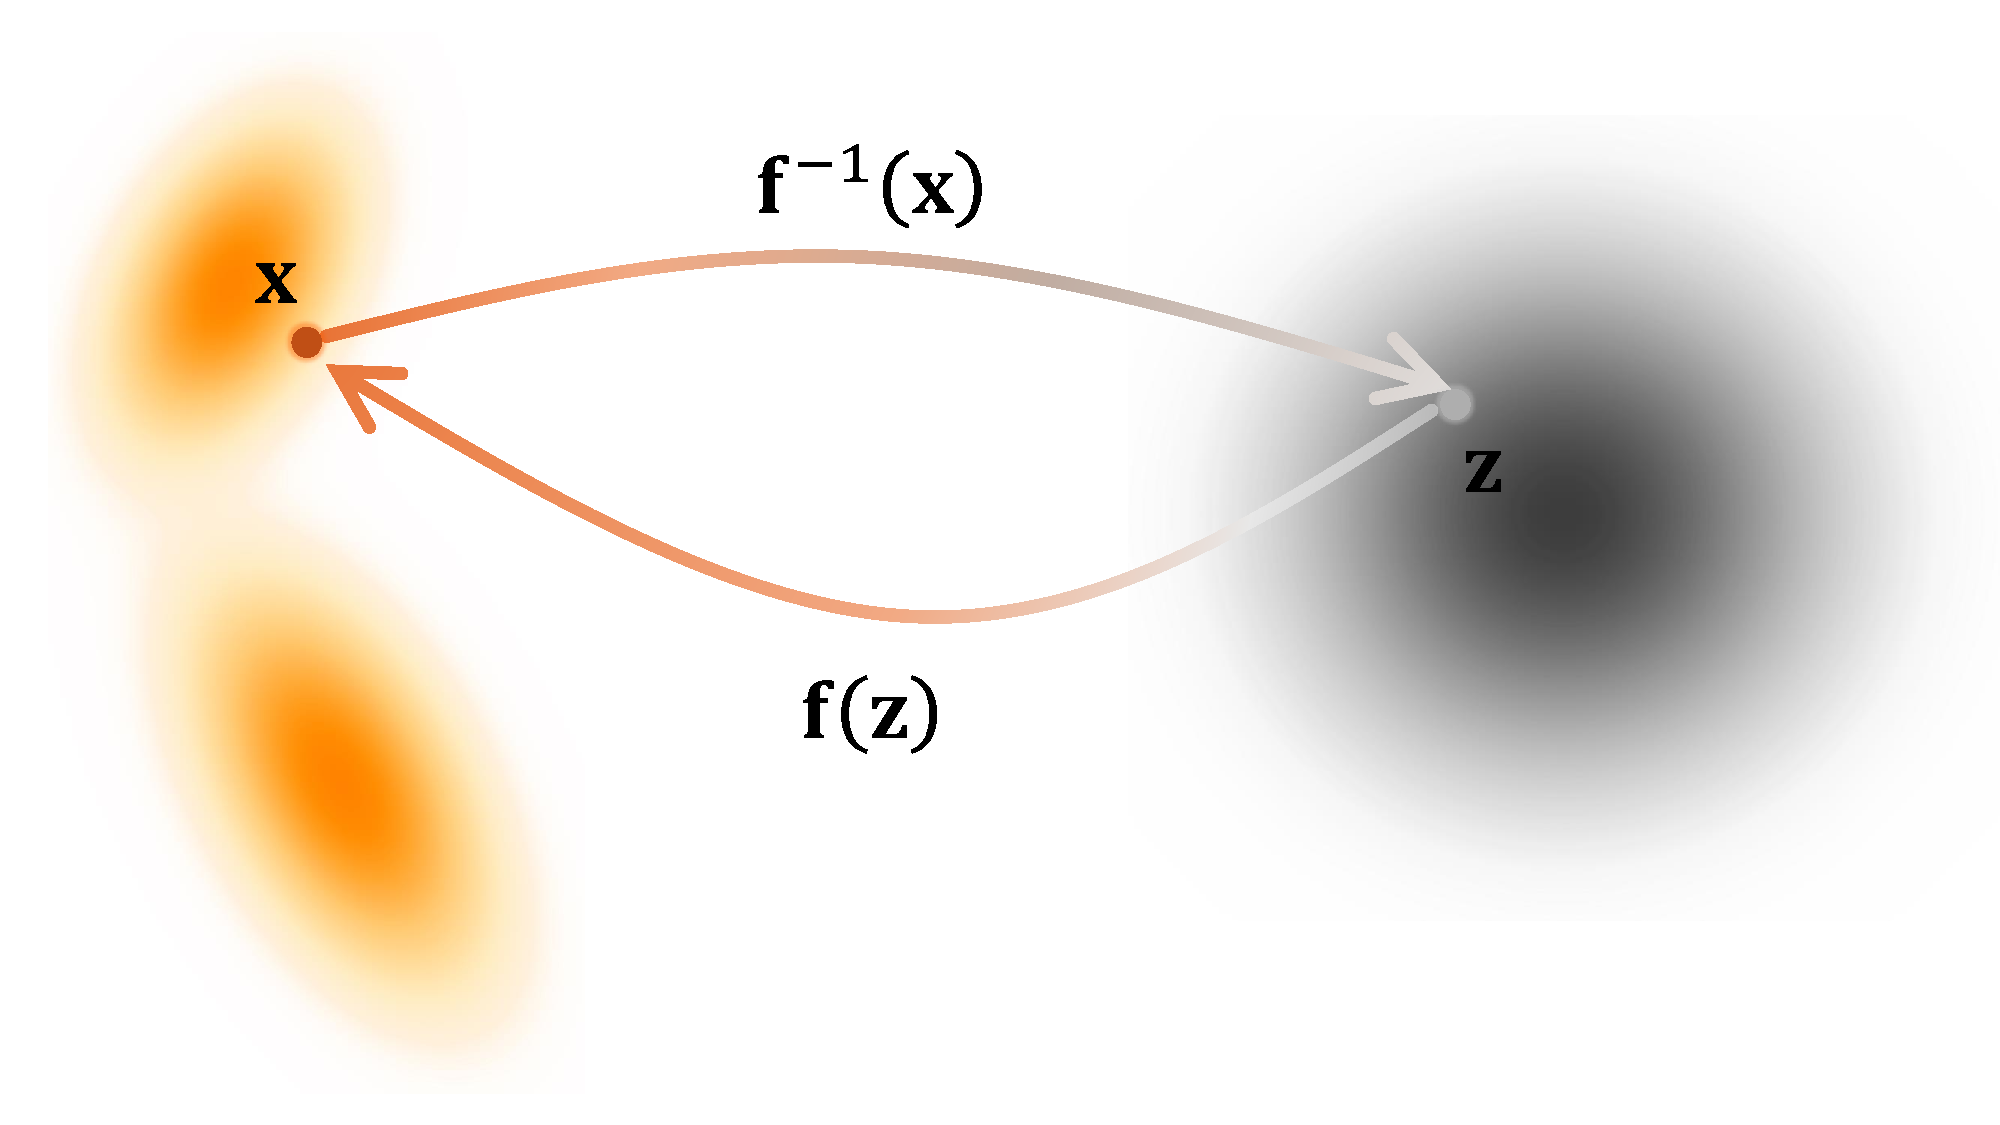
\includegraphics[width=0.9\linewidth]{Images/PartB/flow_density.pdf}
    \caption{\textbfs{可逆映射下 NF 的样本移动示意图。}它由一系列可逆函数 $\rvf: \rvz \mapsto \rvx$ 构成，这些函数将隐变量 $\rvz$ 变换为数据 $\rvx$，同时逆映射 $\rvf^{-1}: \rvx \mapsto \rvz$ 用于重建数据。一个 NF 类似于编码器--解码器结构，但编码器被实现为一个光滑可逆映射，而解码器恰为其逆映射。相应的密度变化可通过变量替换公式计算，如 \Cref{eq:nf-change-of-var} 所示。\figcredit{由作者绘制。}}
    \label{fig:sample-and-change-of-variable}
\end{figure}

\subsection{归一化流}

NF~\citep{rezende2015variational} 通过一个可逆映射将一个简单先验 $p_{\text{prior}}(\rvz)$（例如标准高斯 $\mathcal{N}(\bm{0}, \rmI)$）进行变换，来建模一个复杂数据分布 $p_{\text{data}}(\rvx)$：
\[
\rvf_{\bm{\phi}}: \mathbb{R}^D \to \mathbb{R}^D,
\]
其中 $\rvx = \rvf_{\bm{\phi}}(\rvz)$ 且 $\rvz \sim p_{\text{prior}}$。这里 $\rvx$ 与 $\rvz$ 维数相同。
利用 \Cref{eq:nf-change-of-var} 中的变量替换公式，模型似然为\footnote{若进一步约束该映射为某个凸势函数的梯度，
即 $\rvf_\bphi = \nabla \psi_\bphi$，其中 $\psi_\bphi$ 为凸函数，则
\Cref{eq:nf-change-of-var-log} 退化为 \Cref{eq:monge-ampere} 中的 Monge--Ampère
关系。
该偏微分方程刻画了在二次代价下从一个分布到另一个分布的最优变换。详见 \Cref{ch:ot-eot} 与 \citep{huangconvex}。
}
\begin{align}\label{eq:nf-change-of-var-log}
\log p_{\bm{\phi}}(\rvx) = \log p_{\text{prior}}(\rvz) + \log \left| \det \frac{\partial \rvf_{\bm{\phi}}^{-1}(\rvx)}{\partial \rvx} \right|.
\end{align}




\paragraph{训练目标。}
参数 $\bm{\phi}$ 通过在数据上最大化似然来学习：
\begin{align}\label{eq:nf-training}
\mathcal{L}_{\text{NF}}(\bm{\phi}) = \mathbb{E}_{\rvx \sim p_{\text{data}}} \left[ \log p_{\bm{\phi}}(\rvx) \right].
\end{align}
计算 \Cref{eq:nf-change-of-var-log} 中的雅可比行列式代价可能很高，一般情况下复杂度标度为 $\mathcal{O}(D^3)$。

\paragraph{构造可逆变换。}






单一复杂可逆网络因其雅可比行列式而代价高昂。反之，简单变换（例如线性变换）虽然高效，却缺乏表达能力。


为在二者之间取得平衡，NF 采用一串 $L$ 个可训练的可逆映射 $\{\rvf_k\}_{k=0}^{L-1}$，每个映射都具有可高效计算的雅可比：
\[
\rvf_{\bm{\phi}} = \rvf_{L-1} \circ \rvf_{L-2} \circ \cdots \circ \rvf_0.
\]
每个 $\rvf_k$ 都由一个神经网络参数化，但为简洁起见我们省略对 ${\bm{\phi}}$ 的显式依赖。


样本经如下方式变换：
\begin{align}\label{eq:nf-seq}
\rvx_{k+1} = \rvf_k(\rvx_k), \quad k = 0, \ldots, L-1,
\end{align}
其中 $\rvz=\rvx_0 \sim p_{\text{prior}}$ 且 $\rvx = \rvx_L$ 对应数据。所得的（对数）密度为
\begin{align}\label{eq:multi-nf-density}
\begin{aligned}
    p_{\bm{\phi}}(\rvx) &= p_{\text{prior}}(\rvx_0) \prod_{k=0}^{L-1} \left| \det \frac{\partial \rvf_k}{\partial \rvx_k} \right|^{-1}, \text{ or equivalently,}\\
\log p_{\bm{\phi}}(\rvx) &= \log p_{\text{prior}}(\rvx_0) + \sum_{k=0}^{L-1} \log \left| \det \frac{\partial \rvf_k}{\partial \rvx_k} \right|^{-1}.
\end{aligned}
\end{align}


\vspace{0.3cm}
\begin{figure}[tbh!]
    \centering
\begin{tikzpicture}[
    ->, % Sets default arrow type
    >=Stealth, % Sets default arrowhead style
    node_dist/.style={left=1.7cm of #1}, % Position nodes to the LEFT
    font=\small,
    thick
  ]

  % Define a style for the nodes
  \tikzset{state/.style={
      rectangle,
      rounded corners=3pt,
      draw=black,
      fill=gray!10,
      minimum height=35pt,
      minimum width=25pt
    }
  }

  % Place the nodes from RIGHT to LEFT
  \node[state] (x0) {$\rvx_0 $};
  \node[state] (x1) [node_dist=x0] {$\rvx_1$};
  \node[state] (x2) [node_dist=x1] {$\rvx_2$};
  \node (dots) [left=0.7cm of x2] {$\boldsymbol{\cdots}$};
  \node[state] (xL) [node_dist=dots] {$\rvx_L$};

  % Draw the arrows (edges) with labels
  
  % Top path (Generative, right to left) - Shifted up
  \path [black] ([yshift=4.5pt]x0.west)  edge node[above] {$\rvf_0$} ([yshift=4.5pt]x1.east);
  \path [black] ([yshift=4.5pt]x1.west) edge node[above] {$\rvf_1$} ([yshift=4.5pt]x2.east);
  \path [black] ([yshift=4.5pt]x2.west) edge ([yshift=4.5pt]dots.east);
  \path [black] ([yshift=4.5pt]dots.west) edge node[above, pos=0.4] {$\rvf_{L-1}$} ([yshift=4.5pt]xL.east);
  
  % Bottom path (Inference, left to right) - Shifted down
  \path ([yshift=-4.5pt]x1.east) edge node[below] {$\rvf_0^{-1}$} ([yshift=-4.5pt]x0.west);
  \path ([yshift=-4.5pt]x2.east) edge node[below] {$\rvf_1^{-1}$} ([yshift=-4.5pt]x1.west);
  \path ([yshift=-4.5pt]dots.east) edge ([yshift=-4.5pt]x2.west);
  \path ([yshift=-4.5pt]xL.east) edge node[below, pos=0.6] {$\rvf_{L-1}^{-1}$} ([yshift=-4.5pt]dots.west);

\end{tikzpicture}
\caption{\textbfs{NF 示意图。}一个 NF 由一叠可逆映射
$\rvf_{\bm{\phi}} = \rvf_{L-1} \circ \rvf_{L-2} \circ \cdots \circ \rvf_0$ 构成。
该变换将隐变量样本 $\rvx_0 \sim p_{\mathrm{prior}}$ 映射为数据样本 $\rvx_L \sim p_{\mathrm{data}}$。\figcredit{由作者绘制。}}
    \label{fig:nf-stack}
\end{figure}

\paragraph{可逆流的示例。}已有大量文献聚焦于设计能够高效计算雅可比行列式的单层流构造。下面我们介绍两种具有代表性的类型：平面流~\citep{rezende2015variational} 与残差流~\citep{chen2019residual,behrmann2019invertible}，后者启发了 \Cref{subsec:NODE} 中的发展。
\subparagraph{平面流：}它施加一个简单的变换
\[
\rvf(\rvz) = \rvz + \rvu h(\rvw^\top \rvz + b),
\]
where $\rvu, \rvw \in \mathbb{R}^D$，$b \in \mathbb{R}$，$h(\cdot)$ 是一个激活函数。雅可比行列式为
\[
\left| 1 + \rvu^\top h'(\rvw^\top \rvz + b) \rvw \right|.
\]

\subparagraph{残差流：}
将变换 $\rvf$ 定义为
\begin{align}\label{eq:residual-flow}
\rvf(\rvz) = \rvz + \rvv(\rvz),
\end{align}
其中 $\rvv$ 为压缩映射（Lipschitz 常数 $< 1$）。这由 Banach 不动点定理保证了可逆性。

雅可比的对数行列式可化简为迹展开：
\begin{align}\label{eq:log-det-tr}
    \log \Bigg|\det \frac{\partial \rvf(\rvz)}{\partial \rvz} \Bigg| &= \log \left( \det \frac{\partial \rvf(\rvz)}{\partial \rvz} \right) \nonumber\\
    &= \Tr\left(\log\left(\frac{\partial \rvf(\rvz)}{\partial \rvz}\right)\right) \nonumber\\
    &= \Tr\left(\log\left(\rmI + \frac{\partial \rvv(\rvz)}{\partial \rvz}\right)\right) \nonumber\\
    &= \sum_{k=1}^{\infty} \frac{(-1)^{k+1}}{k} \Tr\left(\left(\frac{\partial \rvv(\rvz)}{\partial \rvz}\right)^k\right),
\end{align}
借助于迹估计量~\citep{hutchinson1989stochastic} 可使计算变得高效。

\paragraph{采样与推断。}
从 NF 中采样非常直接：抽取 $\rvx_0 \sim p_{\text{prior}}$ 并计算 $\rvx = \rvf_{\bm{\phi}}(\rvx_0)$。精确似然可由 \Cref{eq:multi-nf-density} 得到。


\subsection{神经 ODE}\label{subsec:NODE}
\begin{figure}[th!]
    \centering
    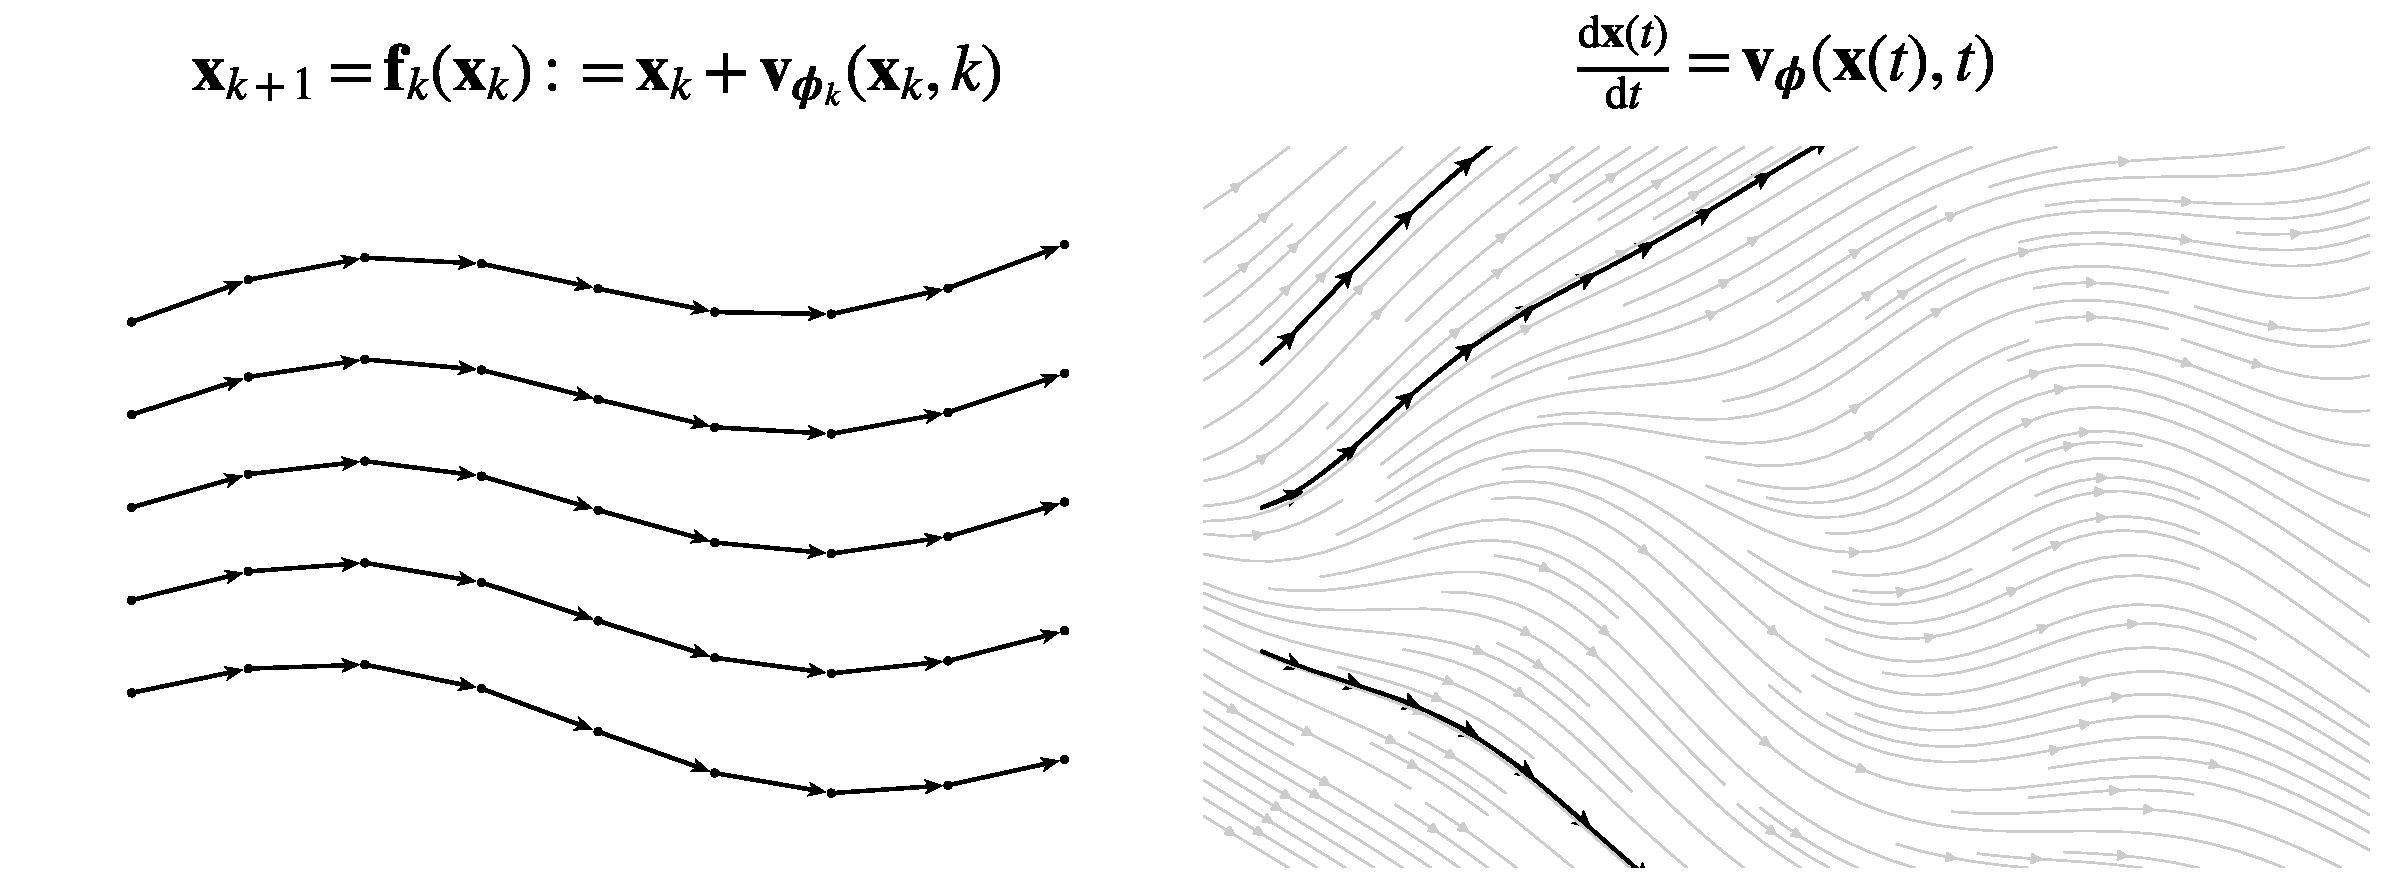
\includegraphics[width=\linewidth]{Images/PartB/discrete_vs_continuous_side_by_side_white.pdf}
    \caption{\textbfs{离散时间与连续时间归一化流的对比。}（左）一个离散 NF 通过有限序列的可逆映射 $\mathbf{x}_{k+1} = \mathbf{f}_k(\mathbf{x}_k)$ 传输样本，
得到分段、不相交的轨迹（带箭头的点）。（右）一个连续 NF（神经 ODE）沿 $\frac{\diff\mathbf{x}(t)}{\diff t} = \mathbf{v}_{\boldsymbol{\phi}}(\mathbf{x}(t),t)$ 的积分曲线演化状态，
其中带切向箭头的黑色路径绘制在灰色向量场之上。\figcredit{由作者绘制。}}
    \label{fig:nf-cnf}
\end{figure}


\paragraph{从离散时间 NF 到连续时间 NF（神经 ODE）。}
NF 通常被表述为一串 $L$ 个离散、可逆的变换。透过 \Cref{eq:nf-seq} 以及 \Cref{eq:residual-flow} 中“残差流”形式的视角，每一层可写成如下形式：
\[
\rvx_{k+1} = \rvf_k(\rvx_k) := \rvx_k + \rvv_{\bm{\phi}_k}(\rvx_k, k),
\]
where $\rvv_{\bm{\phi}_k}(\cdot, k)$ 是一个由神经网络参数化的、与层相关的速度场。直观地讲，这个速度场是一个学习到的向量值函数，它以平滑的小步幅在输入空间中“推动”数据点。每次变换都沿着该速度所提示的方向移动点，逐步将简单的先验分布塑造为复杂的目标分布。


事实上，这一表述恰好对应于带可学习参数 $\bphi$ 的连续时间 ODE 的 Euler 离散化：
\[
\frac{\diff \rvx(t)}{\diff t} = \rvv_{\bm{\phi}}(\rvx(t), t).
\]
 在层数趋于无穷、步长趋于零（$\Delta t \to 0$）的极限下，离散 NF 收敛到一个连续模型，由此得到 \emph{神经 ODE}（NODE）~\citep{chen2018neural} 的框架，也称为 \emph{连续归一化流}（CNF）。



\paragraph{神经 ODE 的形式化设定。}
一个神经 ODE 通过下式定义一个连续变换：
\begin{align}\label{eq:neural-ode}
    \frac{\diff \rvx(t)}{\diff t} = \rvv_{\bm{\phi}}(\rvx(t), t),\quad t\in [0,T]
\end{align}
where:
\begin{itemize}
    \item $ \rvx(t) \in \mathbb{R}^D $ 是 $t$ 时刻的状态；为简洁起见，我们有时写作 $\rvx_t$；
    \item $\rvv_{\bm{\phi}}(\rvx(t), t)$ 是由 $\bm{\phi}$ 参数化的神经网络。
\end{itemize}


\subparagraph{NODE 的目标。}
从初始条件 $\rvx(0) \sim p_{\text{prior}}$ 出发，ODE 随时间连续演化状态，诱导出一族边际分布 $p_{\bm{\phi}}(\rvx_t, t)$（与 PF-ODE 类似！）\footnote{我们采用翻转时间的约定：$t = 0$ 表示先验（源），$t = 1$ 表示数据（目标）分布。先验可交替地写作 $p_{\bm{\phi}}(\rvx(0), 0)$、$p_{\text{prior}}(\rvx(0), 0)$，或简写为 $p_{\text{prior}}(\rvz)$。
}。

目标是学习神经向量场 $\rvv_{\bm{\phi}}$，直观上它表示一个沿数据空间中连续轨迹传输点的速度。通过学习这一速度，$t=T$ 时刻的终端分布将匹配目标分布 $p_{\mathrm{data}}(\cdot)$。这一连续变换将离散归一化流和神经 ODE 统一在同一个框架之中。


\begin{figure}
    \centering
    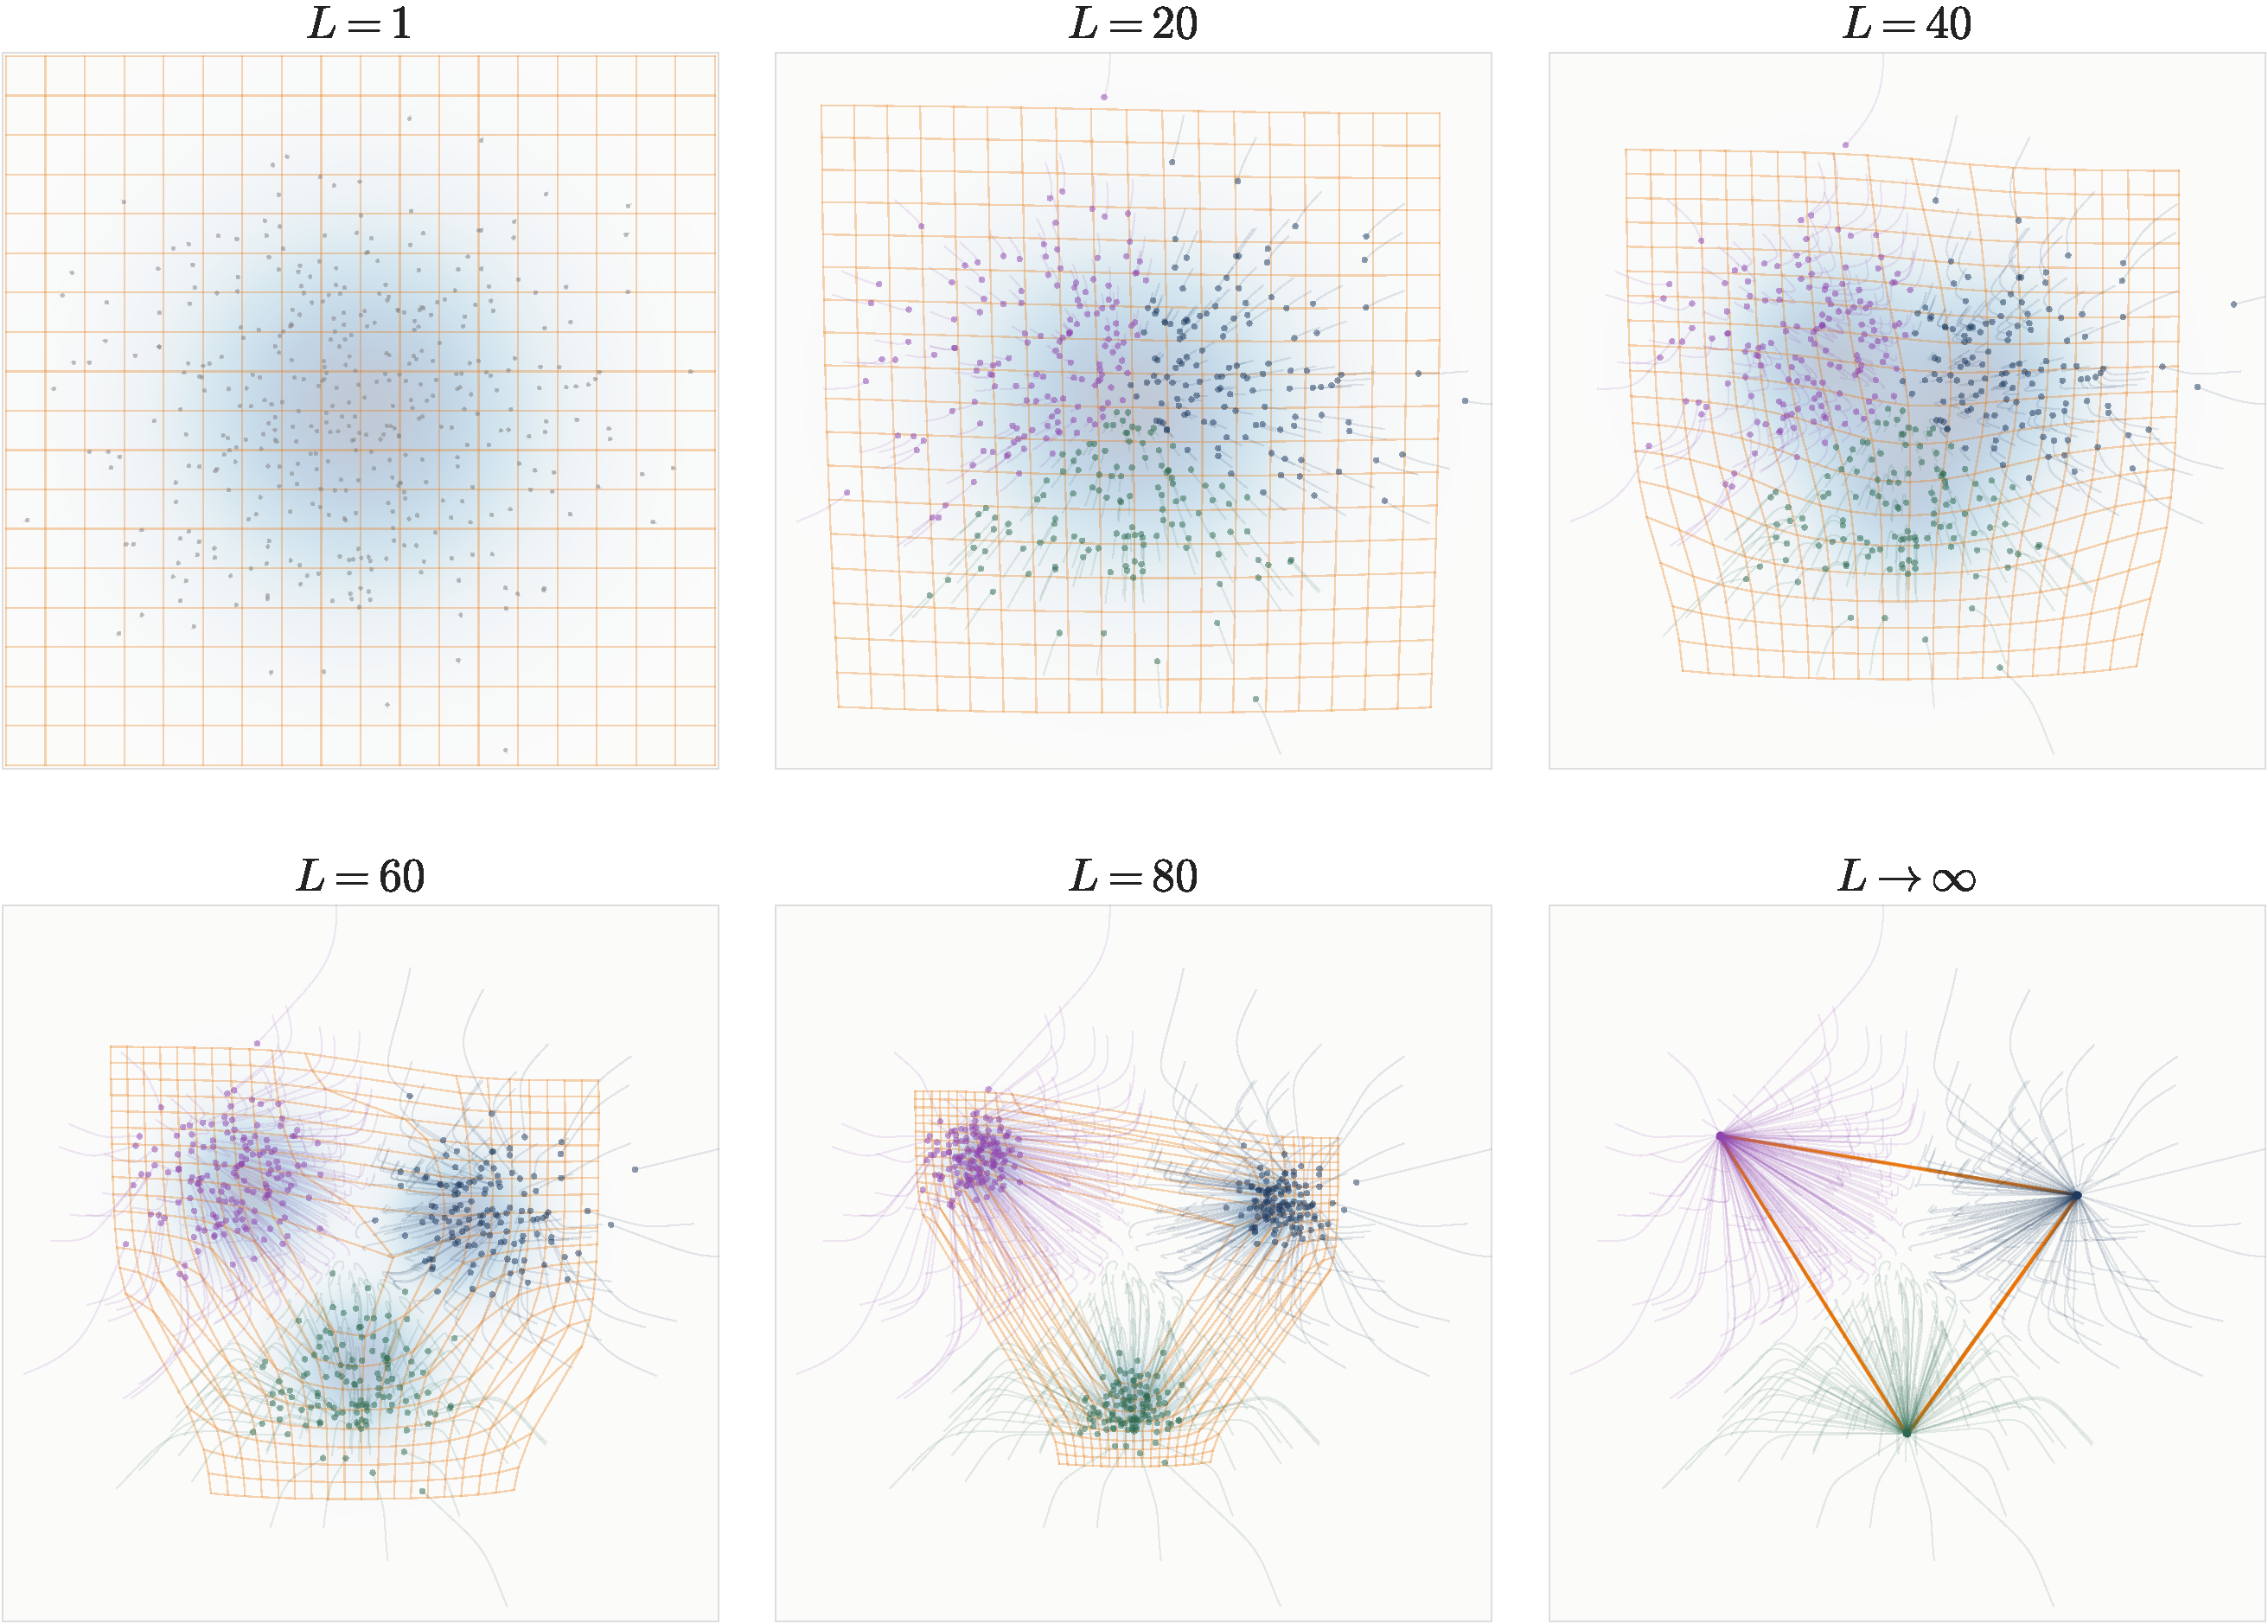
\includegraphics[width=\linewidth]{Images/PartB/cov_2d_layers.pdf}
    \caption{\textbfs{逼近一个连续传输流的离散双射。}
随着双射层数 $L$ 增加，映射复合逐步使样本、潜在分布以及参考网格从源配置变形到目标几何。
当 $L$ 较小时，变换较为粗糙、明显分层；随着 $L$ 增大，变形变得更加平滑、分辨率更高。
在无穷深度的极限下，若按每一层成为一个无穷小变换的标度进行缩放，则堆叠的双射逼近一个连续的、依赖时间的流，所诱导的密度演化由 \Cref{eq:continuity_eq} 中的连续性方程主宰。\figcredit{由作者在 AI 辅助编程下绘制。}}
    \label{fig:bijection-continuity}
\end{figure}



\paragraph{连续时间的变量替换公式。}
类似于 \Cref{eq:nf-change-of-var} 或 \Cref{eq:multi-nf-density}，\citet{chen2018neural} 推导出了变量替换公式的连续时间类比。对于在 \Cref{eq:neural-ode} 下演化的过程 $\rvx(t)$，其依赖于时间的密度 $p_{\bm{\phi}}(\rvx(t), t)$，所谓的 \emph{瞬时变量替换公式} 为：
\[
\frac{\diff}{\diff t} \log p_{\bm{\phi}}(\rvx(t), t) = -\nabla_{\rvx}\cdot\rvv_{\bm{\phi}}(\rvx(t), t).
\]
因此，在给定先验 $p_{\text{prior}}(\rvx(T), T)$ 下，由神经 ODE 诱导的终端状态 $\rvx(T)$ 的对数密度为
\begin{align}\label{eq:NODE-likelihood}
    \log p_{\bm{\phi}}(\rvx(T), T) = \log p_{\text{prior}}(\rvx(0), 0) - \int_0^T \nabla_{\rvx} \cdot \rvv_{\bm{\phi}}(\rvx(t), t)   \mathrm{d}t.
\end{align}
该表达式通过数值求解 ODE 即可实现精确似然计算，进而允许对模型进行最大似然训练。我们稍后将对此详细展开。


尽管初看可能陌生，这个瞬时变量替换公式其实是 Fokker-Planck 方程的一个特例，具体而言是其确定性形式，即所谓的 \emph{连续性方程}（见 \Cref{app:continuity}）。它也可被解释为 \Cref{eq:multi-nf-density} 的连续时间极限。我们将这一结果及其推导总结为如下引理：

\lemp{瞬时变量替换}{instant-change-of-var}{
设 ${\rvz}(t)$ 是一个具有依赖时间的密度 $p({\rvz}(t), t)$ 的连续随机过程，且假设它按如下 ODE 演化：
\begin{align*}
    \frac{\diff \rvz(t)}{\diff t} = \mathbf{F}({\rvz}(t), t).
\end{align*}
假设 $\mathbf{F}$ 在 ${\rvz}$ 上一致 Lipschitz 且关于 $t$ 连续，则对数密度的时间导数满足：
\begin{align}\label{eq:instant-change-of-var}
\frac{\partial \log p({\rvz}(t), t)}{\partial t} = -\nabla_\rvz \cdot \mathbf{F} (\rvz(t), t).
\end{align}
}{我们在 \Cref{app-sec:flow-proof} 中给出两种等价的推导。
}


\subparagraph{与离散时间公式的联系。}
\Cref{eq:NODE-likelihood} 中 NODE 的似然，
\[
\log p_{\bm{\phi}}(\rvx(T), T) = \log p_{\text{prior}}(\rvx(0), 0) - \int_0^T \nabla_\rvx \cdot \rvv_{\bm{\phi}}(\rvx(t), t) \diff t,
\]
可以被视为 \Cref{eq:multi-nf-density} 中离散归一化流公式的连续时间类比：
\[
\log p_{\bm{\phi}}(\rvx_L) = \log p_{\text{prior}}(\rvx_0) - \sum_{k=0}^{L-1} \log \left| \det \frac{\partial \rvf_k}{\partial \rvx_k} \right|.
\]
积分对应于求和，迹算子则取代了对数行列式，正如 \Cref{eq:log-det-tr} 中所讨论的那样。这些对应关系在引理的证明中得到了进一步探讨。

\paragraph{训练 NODE。}
基于 \Cref{eq:NODE-likelihood}，NODE 学习一个参数化的速度场 $\rvv_{\bm{\phi}}$，使得终端分布
\[
p_{\bm{\phi}}(\cdot, T) \approx p_{\text{data}},
\]
其中轨迹从隐变量 $\rvx(0) \sim p_{\text{prior}}$ 出发，经 ODE 流演化。训练遵循 \Cref{eq:MLE} 中的 MLE 框架：
\[
\mathcal{L}_{\text{NODE}}(\bm{\phi}) := \mathbb{E}_{\rvx \sim p_{\text{data}}} \big[\log p_{\bm{\phi}}(\rvx, T)\big].
\]

\subparagraph{精确对数似然计算。}
为了计算数据点 $\mathbf{x}$ 的 $\log p_{\bm{\phi}}(\mathbf{x}, T)$，我们对变量替换公式 \eqref{eq:NODE-likelihood} 进行积分：
\begin{align}
\log p_{\bm{\phi}}(\mathbf{x}, T) = \log p_{\text{prior}}(\mathbf{z}(0)) - \int_0^T \nabla_{\mathbf{z}} \cdot \mathbf{v}_{\bm{\phi}}(\mathbf{z}(t), t) \diff t.
\end{align}
这里 $\mathbf{z}(t)$ 从 $t = T$ 反向求解到 $t = 0$ 的 ODE：
\[
\frac{\diff\mathbf{z}}{\diff t} = \mathbf{v}_{\bm{\phi}}(\mathbf{z}(t), t)
\]
初值取 $\mathbf{z}(T) = \mathbf{x}$。对标准分布而言，先验项 $\log p_{\text{prior}}(\mathbf{z}(0))$ 是易处理的。这使得神经 ODE 中可以进行精确的、基于似然的训练与评估。

\subparagraph{基于梯度的优化。}
最大化 $\mathcal{L}_{\text{NODE}}$ 需要通过 ODE 求解器进行反向传播。伴随灵敏度方法~\citep{pontryagin2018mathematical, chen2018neural} 通过一个辅助 ODE 来计算梯度，具有 $\mathcal{O}(1)$ 的内存复杂度，但由于每一步都需要数值积分，NODE 的训练仍然代价高昂。

\paragraph{用 NODE 进行推断。}
用训练好的模型 $\rvv_{\bm{\phi}^\times}$ 进行采样，需抽取 $\rvx(0) \sim p_{\text{prior}}$ 并向前积分（借助数值求解器）：
\[
\rvx(T) = \rvx(0) + \int_0^T \rvv_{\bm{\phi}^\times}(\rvx(t), t)   \diff t.
\]
终端状态 $\rvx(T)$ 近似为来自 $p_{\text{data}}$ 的一个样本。

此外，我们注意到对于任意向量场 $\rmF$，下述恒等式成立：
\[
    \Tr\left(\frac{\partial \rmF}{\partial \rvz(t)} \right) = \nabla_{\rvz} \cdot \rmF.
\]
因此，散度可以借助随机迹估计量（例如 Hutchinson 估计量~\citep{hutchinson1989stochastic}）进行高效估计，这使得在高维情形下精确似然计算变得更加可行。


% \subsection{Closing Remarks}\label{subsec:remark-flow}
%  We first compare NODEs with discrete NFs, then outline their connection to diffusion models.
% \paragraph{Advantages of NODEs over Discrete NFs.}
% NODEs offer two key advantages:
% \begin{enumerate}
%     \item \textbfs{Flexible Architectures:} Unlike discrete NFs, NODEs do not require invertible transformations, as ODE solutions are guaranteed under Lipschitz conditions on the velocity field $\rvv_{\bm{\phi}}$.
%     \item \textbfs{Efficient Likelihoods Computation:} NODEs compute divergence $\nabla \cdot \rvv_{\bm{\phi}}$ with $\mathcal{O}(D)$ complexity, compared to the $\mathcal{O}(D^3)$ Jacobian determinant in discrete NFs, enabling high-dimensional scalability.
% \end{enumerate}
% Beyond generative modeling, NODEs are also used in dynamical systems, time series, and mathematical physics~\citep{kidger2022neural}.


% \paragraph{What Lies Ahead?}
% In this section, we have examined the development of NFs and NODEs:
% \begin{itemize}
%     \item \textbfs{Stage 1.} Single-layer invertible transformations in NFs;
%     \item \textbfs{Stage 2.} Multiple layers of invertible transformations in NFs;
%     \item \textbfs{Stage 3.} Continuous-time extension through NODEs, equivalent to infinitely many layers of invertible transformations.
% \end{itemize}

% It is fascinating to see how the evolution of flow-based models echoes that of VAEs~(\Cref{ch:variational}) and score-based methods~(\Cref{ch:score-based}). Each of these modeling paradigms embarks on a similar journey: beginning with simple, discrete-time, single-layer structures, advancing to deeper multi-layer designs (e.g., DDPM/NCSN), and ultimately converging toward elegant continuous-time formulations (Score SDE).

% However, a crucial difference emerges: even though diffusion models are associated with an ODE (i.e., PF-ODE), they do not directly learn an arbitrary velocity field $\mathbf{v}_{\bm{\phi}}$ as in NODEs. Instead, diffusion models learn objectives (e.g., score) that define ODEs aimed at matching prescribed marginal distributions--governed by Fokker-Planck equation. This approach makes diffusion model training simulation-free and thus computationally efficient, in contrast to NODEs which require solving numerical ODEs during training.

% Flow matching inherits this essential characteristic of diffusion model training and resolves the simulation bottleneck of NODEs, enabling efficient distribution-to-distribution transport via ODEs with prescribed underlying structure. We will explore this further in the next chapter.




\newpage
\clearpage
\section{\texorpdfstring{流匹配框架}{Flow Matching Framework}}\label{sec:flow-matching-framework}

Score SDE~（\Cref{ch:score-sde}）与 NODE~（\Cref{sec:flow-based-method}）为生成建模提供了一种替代视角：学习一个连续时间的流（随机或确定），将一个简单的高斯先验样本 $\bm{\epsilon} \sim p_{\text{prior}}$ 传输为来自 $p_{\text{data}}$ 的类数据样本。

\emph{流匹配}（FM）框架~\citep{lipman2022flow,lipman2024flow,tongimproving} 在这一思想之上展开，并将其推广为学习两个 \emph{任意} 固定端点分布之间的流：一个源分布 $p_{\text{src}}$ 和一个目标分布 $p_{\text{tgt}}$，并假定二者都易于采样。在这一更宽泛的设定中，生成任务成为 $p_{\text{src}}$ 为高斯先验、$p_{\text{tgt}}$ 为数据分布时的特例。

本节我们采用 FM 的视角\footnote{若干相关方法都共享用连续时间流在端点分布之间进行传输这一核心思想，只是表述略有不同。这些方法包括流匹配（FM）~\citep{lipman2022flow,neklyudov2023action}、整流流（RF）~\citep{liu2022rectified,heitz2023iterative} 和随机插值~\citep{albergo2023stochastic,albergobuilding,ma2024sit}。这里我们采用 FM 的术语作为一种统一的表示。}，强调其核心原理：学习一个依赖时间的向量场 $\mathbf{v}_t(\rvx_t)$，使与之对应的 ODE 流在满足边界条件
\[
p_0 = p_{\text{src}}, \quad p_1 = p_{\text{tgt}}.
\]
When $p_{\text{src}}$ 为高斯分布时，我们称这一设定为 \emph{高斯流匹配}。与经典扩散模型相比，FM 仅利用端点处的样本即可实现针对一大类传输问题的高效、免仿真训练。






\subsection{来自基于分数方法的启示}\label{subsec:lesson-score}

我们用一种略有不同但等价的表述重新审视 Score SDE 框架（\Cref{ch:score-sde}），从中提炼出激发 FM 方法的关键见解。这一分析揭示了扩散模型如何隐式地学习概率流，并启发了更直接的表述形式。


\paragraph{第一步：定义条件路径及其边际密度。}

\begin{figure}[th!]
    \centering
    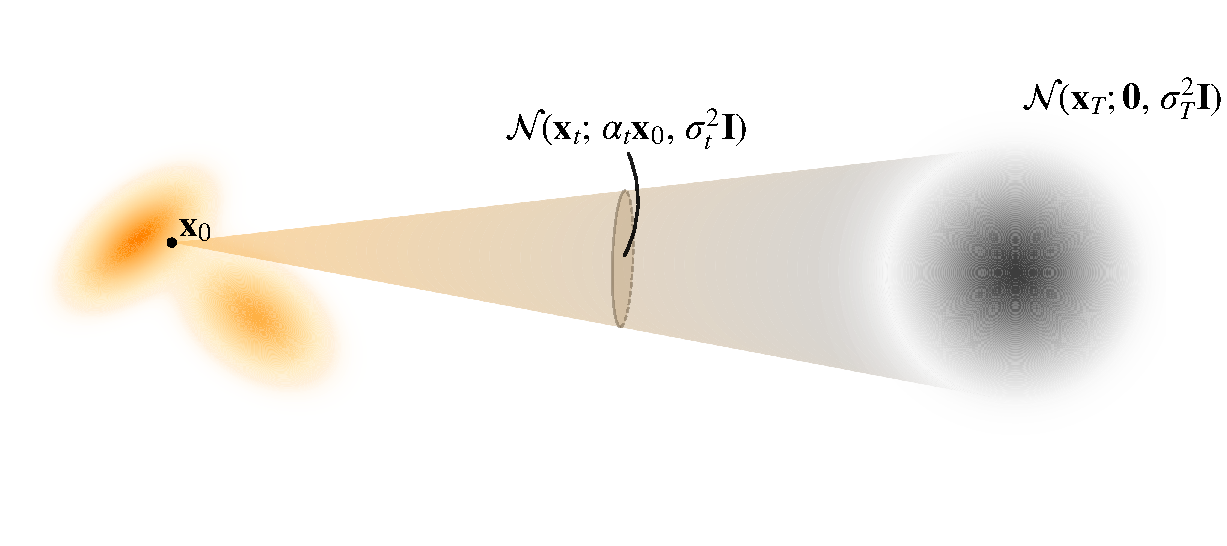
\includegraphics[width=\linewidth]{Images/PartB/data_vs_prior_cone_with_oval.pdf}
    % \vspace{-1.5cm}
    \caption{\textbfs{条件转移分布示意图。}
$p_t(\rvx_t | \rvx_0) = \mathcal{N}(\rvx_t;\alpha_t \rvx_0,\sigma_t^2 \mathbf{I})$，
定义了一条（高斯）条件概率路径，从数据样本
$\rvx_0 \sim p_{\text{data}}$（左）通向高斯先验
$p_{\text{prior}}$（右）。\figcredit{由作者绘制。}}
    \label{fig:data-prior-conditioning}
\end{figure}

一个扩散模型指定了一个连续时间的密度族 $\{p_t\}_{t \in [0,1]}$，它在 $t=1$ 处将一个简单先验 $p_{\text{prior}}$（例如高斯）作为源，传输到 $t=0$ 处的目标数据分布 $p_{\text{data}}$：
\[
p_1(\rvx_1) = p_{\text{prior}}(\rvx_1), \quad p_0(\rvx_0) = p_{\text{data}}(\rvx_0).
\]
该路径通过前向条件分布隐式定义：
\begin{align}\label{eq:lesson-dm-conditional-path}
    p_t(\rvx_t|\rvx_0) = \mathcal{N}(\rvx_t; \alpha_t \rvx_0, \sigma_t^2 \mathbf{I}), \quad \rvx_0\sim p_{\text{data}}
\end{align}
它诱导出边际密度
\[
p_t(\rvx_t) := \int p_t(\rvx_t |\rvx_0)  p_{\text{data}}(\rvx_0) \mathrm{d}\rvx_0.
\]
条件高斯方差 $\sigma_t^2$ 的增长驱动 $p_t$ 向高斯先验演化。

\paragraph{第二步：速度场。}
边际密度 $p_t$ 的时间演化由一个速度场 $\rvv_t : \mathbb{R}^D \to \mathbb{R}^D$ 主宰，它由 Fokker-Planck 方程导出：
\begin{align}\label{eq:dm-velocity}
    \rvv_t(\rvx) := f(t)\rvx - \frac{1}{2}g^2(t)\nabla_{\rvx} \log p_t(\rvx),
\end{align}
which defines a deterministic particle flow through the PF-ODE:
\[
\frac{\diff \rvx(t)}{\diff t} = \underbrace{f(t)\rvx(t) - \frac{1}{2}g^2(t)\nabla_{\rvx} \log p_t\big(\rvx(t)\big)}_{\rvv_t(\rvx(t))}.
\]
该 ODE 将初始随机变量 $\rvx(0) \sim p_{\text{data}}$ 在时间上向前传输，或将 $\rvx(1) \sim p_{\text{prior}}$ 在时间上向后传输，使得 $\rvx(t)$ 的演化边际密度在每一个 $t \in [0,1]$ 上都匹配 $p_t$（见下文“底层规则”）。

标量函数 $f(t)$ 和 $g(t)$ 由相应前向 SDE 的系数决定，或者等价地由条件路径中定义的高斯核参数 $\alpha_t$ 和 $\sigma_t$ 决定（见 Lemma~\ref{forward-sde}）。


\paragraph{第三步：通过条件策略进行学习。}
目标是用一个神经网络 $\rvs_{\bm{\phi}}(\rvx_t, t)$ 来逼近神谕速度场 $\rvv_t(\rvx_t)$，训练目标为期望平方误差：
\[
\mathcal{L}_{\text{SM}}({\bm{\phi}}) = \mathbb{E}_{t \sim \mathcal{U}[0,1],  \rvx_t \sim p_t} \left[ \left\| \rvs_{\bm{\phi}}(\rvx_t, t) - \nabla_{\rvx_t} \log p_t(\rvx_t) \right\|^2 \right].
\]
由于边际分数 $\nabla_{\rvx_t} \log p_t(\rvx_t)$ 不可获取，我们利用易处理的条件分布来定义条件速度：
\[
\rvv_t(\rvx_t|\rvx_0) := f(t)\rvx_t - \frac{1}{2}g^2(t) \nabla_{\rvx_t} \log p_t(\rvx_t|\rvx_0).
\]
由全期望公式，边际分数可恢复为
\begin{align}\label{eq:marginal-oracle-score}
    \nabla_{\rvx_t} \log p_t(\rvx_t) = \mathbb{E}_{\rvx_0 \sim p(\cdot| \rvx_t)} \left[ \nabla_{\rvx_t} \log p_t(\rvx_t|\rvx_0) \right].
\end{align}
这为如下的替代训练目标提供了依据：
\[
\mathcal{L}_{\text{SM}}({\bm{\phi}}) = \underbrace{\mathbb{E}_{t,  \rvx_0 \sim p_{\text{data}},  \rvx_t \sim p_t(\cdot|\rvx_0)} \left[ \left\| \rvs_{\bm{\phi}}(\rvx_t, t) - \nabla_{\rvx_t} \log p_t(\rvx_t|\rvx_0) \right\|^2 \right]}_{\mathcal{L}_{\text{DSM}}({\bm{\phi}})} + C,
\]
其中 $C$ 是与 ${\bm{\phi}}$ 无关的常数。最小化子 $\rvs^*(\rvx_t, t)$ 满足
\[
\rvs^*(\rvx_t, t) = \mathbb{E}_{\rvx_0 \sim p(\cdot| \rvx_t)} \left[ \nabla_{\rvx_t} \log p_t(\rvx_t|\rvx_0) \right] = \nabla_{\rvx_t} \log p_t(\rvx_t),
\]
其中第二个等号由 \Cref{eq:marginal-oracle-score} 得到，从而验证了条件训练目标的正确性。

\begin{figure}
    \centering
    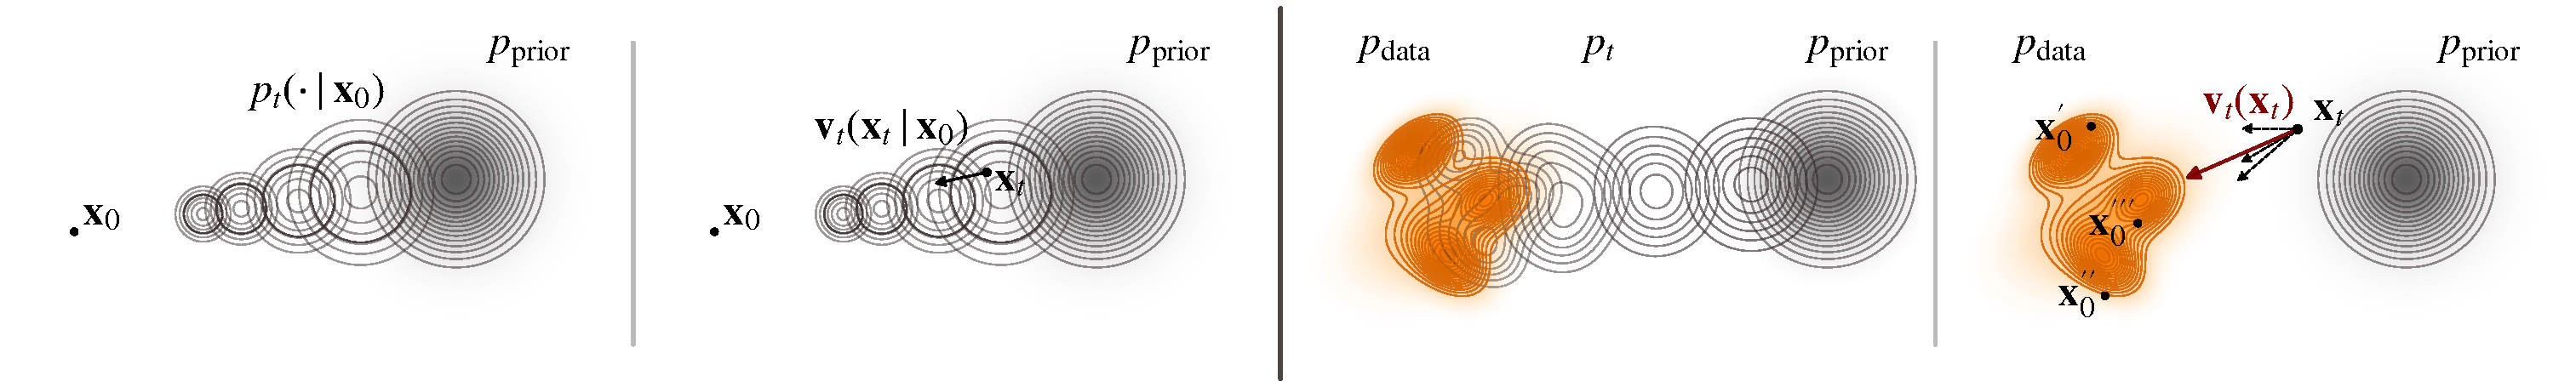
\includegraphics[width=\linewidth]{Images/PartB/four_panel_simple.pdf}
    \caption{\textbfs{扩散中条件视角与边际视角示意图。}（本图受 \citet{lipman2024flow} 启发。）
（1）条件高斯路径 $p_t(\cdot|\mathbf{x}_0)$，展示从一个固定 $\mathbf{x}_0$ 向先验不断扩张的密度。
（2）条件速度 $\mathbf{v}_t(\mathbf{x}_t|\mathbf{x}_0)=f(t)\rvx_t - \tfrac{1}{2}g^2(t) \nabla_{\rvx_t} \log p_t(\rvx_t|\rvx_0)$。
（3）边际密度 $p_t$，将数据分布 $p_{\mathrm{data}}$（橙色）传输为先验 $p_{\mathrm{prior}}$（灰色）。
（4）边际速度 $\mathbf{v}_t(\mathbf{x}_t)=f(t)\rvx_t - \tfrac{1}{2}g^2(t) \nabla_{\rvx_t} \log p_t(\rvx_t)$，由 $\mathbf{x}_t$ 到多个可能起点（虚线）的条件方向取平均得到，结果为红色箭头。在采用单侧条件 $\rvz=\rvx_0$ 的 FM 框架中，
相同的示意图也适用于 $\rvv_t(\rvx_t|\rvx_0)$ 与 $\rvv_t(\rvx_t)$，
无需将它们显式地写成
$\nabla_{\rvx_t}\log p_t(\rvx_t|\rvx_0)$ 或 $\nabla_{\rvx_t}\log p_t(\rvx_t)$ 这些分数的形式。
\figcredit{由作者绘制。}}
    \label{fig:conditional-marginal}
\end{figure}

\paragraph{底层规则：Fokker–Planck 方程。}
边际密度 $p_t$ 按 Fokker–Planck 方程演化：
\begin{mdframed}
\begin{align*}
    \frac{\partial p_t(\rvx)}{\partial t} + \nabla \cdot \Bigg( \underbrace{\left(f(t)\rvx - \frac{1}{2}g^2(t) \nabla_\rvx \log p_t(\rvx)\right)}_{\rvv_t(\rvx)}  p_t(\rvx) \Bigg) = 0.
\end{align*}
\end{mdframed}
该偏微分方程保证了 PF-ODE 给出的密度与前向 SDE 的边际分布相匹配。
为看清这一点，回顾 \Cref{eq:flow-map-def} 中所定义的 PF-ODE 的 \emph{流映射} $\bPsi_{s \to t}(\rvx_s)$，它将 $s$ 时刻的初始状态 $\rvx_s$ 直接携带至其在 $t$ 时刻的状态。
从 $t=1$ 反向运行 PF-ODE 到 $t=0$，以 $\rvx_1 \sim p_{\mathrm{prior}}$ 为初值，我们通过前推公式得到依赖时间的密度：
\begin{align}\label{eq:pushforward-ode}
    p_t^{\mathrm{rev}}(\rvx)
    = \int \delta \left(\rvx - \bPsi_{1 \to t}(\rvx_1)\right) 
      p_{\mathrm{prior}}(\rvx_1) \mathrm{d}\rvx_1.
\end{align}

Fokker–Planck 方程保证所诱导的密度路径与同一演化密度相一致：
\begin{align}\label{eq:p_t-fwd-rev}
p_t^{\mathrm{rev}} = p_t.
\end{align}
特别地，这蕴含了 $p_0^{\mathrm{rev}} = p_0 = p_{\text{data}}$，从而在 $t=0$ 时刻恢复数据分布。由于 ODE 的解映射是双向的，我们也可以类似地从
$\rvx_0 \sim p_{\text{data}}$ 出发并向前求解 ODE，从而进行平行的分析。


\subsection{流匹配框架}\label{subsec:fm-framework}

\Cref{subsec:lesson-score} 的分析表明，扩散模型之所以成功，是因为它学习到了一个在分布之间进行传输并同时满足边界条件的速度场，具体而言就是分数。\Cref{eq:lesson-dm-conditional-path} 中设计的高斯条件路径，其方差 $\sigma_t^2$ 不断增长，隐式地把一个端点锚定在高斯先验上，同时允许条件密度定义在整个空间之上，从而使得基于分数的梯度计算成为可能。

本小节中，我们介绍 FM 框架，它建立在这一见解之上
（\Cref{fig:conditional-marginal} 中的同一示意图也适用于 FM 框架）
并将其推广为学习在两个任意分布
$p_{\text{src}}$ 与 $p_{\text{tgt}}$ 之间传输样本的连续流。





\paragraph{第一步：定义条件路径及其边际密度。}
考虑 $\mathbb{R}^D$ 上的任意源分布和目标概率分布 $ p_{\mathrm{src}} $ 和 $ p_{\mathrm{tgt}} $。我们令\footnote{为了与 FM 文献中的标准记号一致，相对于前面章节我们将时间轴反向：$t=0$ 对应源分布，$t=1$ 对应目标分布。}
\begin{align}\label{eq:marginal-endpoint}
    p_0(\mathbf{x}) = p_{\mathrm{src}}(\mathbf{x}), \quad p_1(\mathbf{x}) = p_{\mathrm{tgt}}(\mathbf{x}).
\end{align}

FM 隐式地定义了一个连续的中间密度族 $\{ p_t \}_{t \in [0,1]}$，在这些端点之间进行插值。每个边际 $ p_t $ 通过一个取自已知分布 $\pi(\mathbf{z})$ 的隐变量 $\mathbf{z}$ 以及一个条件分布 $p_t(\mathbf{x}_t | \mathbf{z})$ 来表示：
\begin{equation}\label{eq:p_t}
    p_t(\mathbf{x}_t) = \int p_t(\mathbf{x}_t | \mathbf{z}) \pi(\mathbf{z}) \diff \mathbf{z},
\end{equation}
其中 $(\pi(\mathbf{z}), \{p_t(\cdot|\mathbf{z})\})$ 的选取满足 \Cref{eq:marginal-endpoint} 中的边界条件。

我们注意到，一般而言边际密度 $p_t$ 是不易处理的，因为它们需要在 $\pi(\mathbf{z})$ 上积分，并且 $\pi(\mathbf{z})$ 与条件分布 $p_t(\mathbf{x}_t|\mathbf{z})$ 都可能很复杂。
尽管如此，对隐变量 $\mathbf{z}$ 加以条件化，赋予了 FM 灵活性去建模一大类超越 \Cref{subsec:lesson-score} 讨论范围的插值路径。$\mathbf{z}$ 的常见选择包括：
\begin{itemize}
    \item \textbfs{双侧条件：} $\mathbf{z} = (\mathbf{x}_0, \mathbf{x}_1) \sim p_{\text{src}}(\mathbf{x}_0) p_{\text{tgt}}(\mathbf{x}_1)$，其中 $\pi$ 将源分布和目标分布耦合在一起。这使得 FM 能够定义任意分布之间的传输。
    \item \textbfs{单侧条件：} $\mathbf{z} = \mathbf{x}_0$ 或 $\mathbf{z} = \mathbf{x}_1$。当源分布选为高斯时，这一情形尤其恢复了类似扩散的设定。
\end{itemize}

在所有情形中，条件分布 $ p_t(\mathbf{x}_t|\mathbf{z}) $ 都应具有易处理的闭式表达。我们在全文中沿用此假设，并在 \Cref{subsec:fm-instantiations} 中给出具体构造，同时在 \Cref{fig:conditional-path} 中给出示意图。


\paragraph{第二步：速度场。}
在标准扩散模型或高斯 FM 中，中间密度族 $\{p_t\}_{t \in [0,1]}$ 在构造时将其中一个端点设为标准高斯。在这一设定下，速度场 $\mathbf{v}_t$ 被唯一确定，并具有与分数相关的闭式表达（见 \Cref{eq:dm-velocity}）。

相比之下，一般的 FM 在一般的源分布和目标分布 $p_{\text{src}}$ 与 $p_{\text{tgt}}$ 之间进行插值，此时速度场不再被唯一确定（后文将解释）。

目标是寻找一个速度场 $\mathbf{v}_t(\mathbf{x})$，使得由此诱导的、能够实现逐样本变换的 ODE
\[
\frac{\diff \mathbf{x}(t)}{\diff t} = \mathbf{v}_t(\mathbf{x}(t)), \quad t \in [0,1],
\]
在每个时刻 $t$，无论从 $\mathbf{x}(0) \sim p_{\text{src}}$ 向前积分还是从 $\mathbf{x}(1) \sim p_{\text{tgt}}$ 向后积分，所产生的 $\mathbf{x}(t)$ 的边际分布都与 $ p_t$ 匹配（更形式化的讨论见 \Cref{subsec:fm-theory}）。

这一要求由 \emph{连续性方程}\footnote{即 Fokker–Planck 方程的确定性类比，不含扩散项。}刻画：
\begin{mdframed}
\begin{equation}\label{eq:continuity_eq}
    \frac{\partial p_t(\mathbf{x})}{\partial t} + \nabla \cdot \big( \mathbf{v}_t(\mathbf{x}) p_t(\mathbf{x}) \big) = 0.
\end{equation}
\end{mdframed}

任何满足 \Cref{eq:continuity_eq} 的速度场 $\mathbf{v}_t$，
都保证 ODE 流以精确地遵循
预定义 $p_t$ 的方式传输样本（详见 \Cref{subsec:fm-theory}）。
因此，求解该 ODE 即可实现从 $p_{\text{src}}$ 到
$p_{\text{tgt}}$ 的传输，同时匹配所有中间分布。

直观上，许多不同的流都可以诱导相同的边际演化。
这是因为 \Cref{eq:continuity_eq} 是一个标量方程，而
$\mathbf{v}_t$ 是 $\mathbb{R}^D$ 中的向量场，因此该方程有无穷多解。
例如，如果 $\mathbf{v}_t$ 解该方程，那么
\[
\mathbf{v}_t + \frac{1}{p_t} \tilde{\mathbf{v}}_t,
\]
也解该方程，其中 $\tilde{\mathbf{v}}_t$ 为任意无散向量场（即
$\nabla \cdot \tilde{\mathbf{v}}_t = 0$）。因此 FM 寻求一个特定的速度场 $\mathbf{v}_t$，
使其满足 \Cref{eq:continuity_eq}，从而实现沿路径 $\{p_t\}$ 的样本连续传输。
然而，对于任意分布，
$p_t$ 与 $\mathbf{v}_t$ 一般没有闭式表达。
作为一个具体示例，我们在 \Cref{subsec:special-fm-instantiations} 中
考虑高斯到高斯的桥，此时两者都可以显式计算。





\paragraph{第三步：通过条件策略进行学习。}
FM 训练的目标是用一个神经网络 $\rvv_{\bm{\phi}}$ 逼近神谕速度场 $\rvv_t$，通过最小化期望平方误差实现：
\[
\mathcal{L}_{\mathrm{FM}}(\bm{\phi}) = \mathbb{E}_{t, \rvx_t \sim p_t} \left[ \left\| \rvv_{\bm{\phi}}(\rvx_t, t) - \rvv_t(\rvx_t) \right\|^2 \right].
\]
我们将这种神经网络参数化称为 \emph{$\rvv$-预测}（速度预测），其目的是直接学习 ODE 的漂移项。

如同 \Cref{subsec:lesson-score} 中那样，神谕速度 $\rvv_t(\rvx)$ 一般是不可处理的。为此，我们引入隐变量 $\rvz \sim \pi(\rvz)$ 并通过构造定义一个条件速度场 $\rvv_t(\rvx |\rvz)$。这允许我们借助全期望公式将损失改写为\footnote{这遵循标准的分部积分论证，正如 \Cref{eq:score-matching} 推导中所用。类似地，\Cref{eq:minimum_velocity} 在分数匹配框架内采用相同的方法推导得到。
}：
\begin{mdframed}
    \begin{align}\label{eq:fm-cfm}
    \mathcal{L}_{\mathrm{FM}}(\bm{\phi}) 
    &= \underbrace{\mathbb{E}_{t, \rvz \sim \pi(\rvz), \rvx_t \sim {\color{orange}p_t(\cdot |\rvz)}} \left[ \left\| \rvv_{\bm{\phi}}(\rvx_t, t) - {\color{orange}\rvv_t(\rvx_t |\rvz)} \right\|^2 \right]}_{\mathcal{L}_{\mathrm{CFM}}(\bm{\phi})} + C,
\end{align}
\end{mdframed}
其中 $C$ 是与 $\bm{\phi}$ 无关的常数。主项 $\mathcal{L}_{\mathrm{CFM}}$ 被称为 \emph{条件流匹配}。

也就是说，最小化 $\mathcal{L}_{\mathrm{FM}}(\bm{\phi})$ 等价于最小化 $\mathcal{L}_{\mathrm{CFM}}(\bm{\phi})$，而后者提供了更易处理的形式。
要让 $\mathcal{L}_{\mathrm{CFM}}(\bm{\phi})$ 实现易处理的、免仿真训练，必须满足两个要求：
\begin{itemize}
    \item[(i)] 从条件概率路径 $p_t(\rvx_t| \rvz)$ 中采样应当简单直接（免仿真）。
    \item[(ii)] 用作回归目标的条件速度 $\rvv_t(\rvx_t| \rvz)$ 必须具有简单的闭式表达。
\end{itemize}
我们将在 \Cref{subsec:fm-instantiations} 中给出满足这些条件的显式构造。这种条件视角使得训练变得可行：模型学习的不是难以处理的无条件速度场 $\rvv_t(\cdot)$，而是易处理的条件速度场 $\rvv_t(\cdot| \rvz)$：这与去噪分数匹配直接类似。


尽管存在无穷多个与给定 $p_t$ 相容的无条件速度场，但其中一个可以通过对条件速度场取边际得到：
\begin{align}\label{eq:marginal-oracle-velocity}
\rvv_t(\rvx_t) &:= \mathbb{E}_{\rvz \sim p(\cdot|\rvx_t)} \left[ \rvv_t(\rvx_t|\rvz)\right],
\end{align}
其中期望是在 $p(\rvz|\rvx_t)$ 上取的。
我们可以证明 \Cref{eq:fm-cfm} 中条件流匹配目标的最小化子 $\rvv^*$ 恢复了这一边际速度：
\begin{align}\label{eq:minimum_velocity}
    \rvv^*(\rvx_t, t) = \rvv_t(\rvx_t).
\end{align}
因此，学习匹配条件速度场 $\rvv_t(\cdot|\rvz)$ 即足以恢复一个有效的无条件速度场。

\begin{figure}[th!]
    \centering
    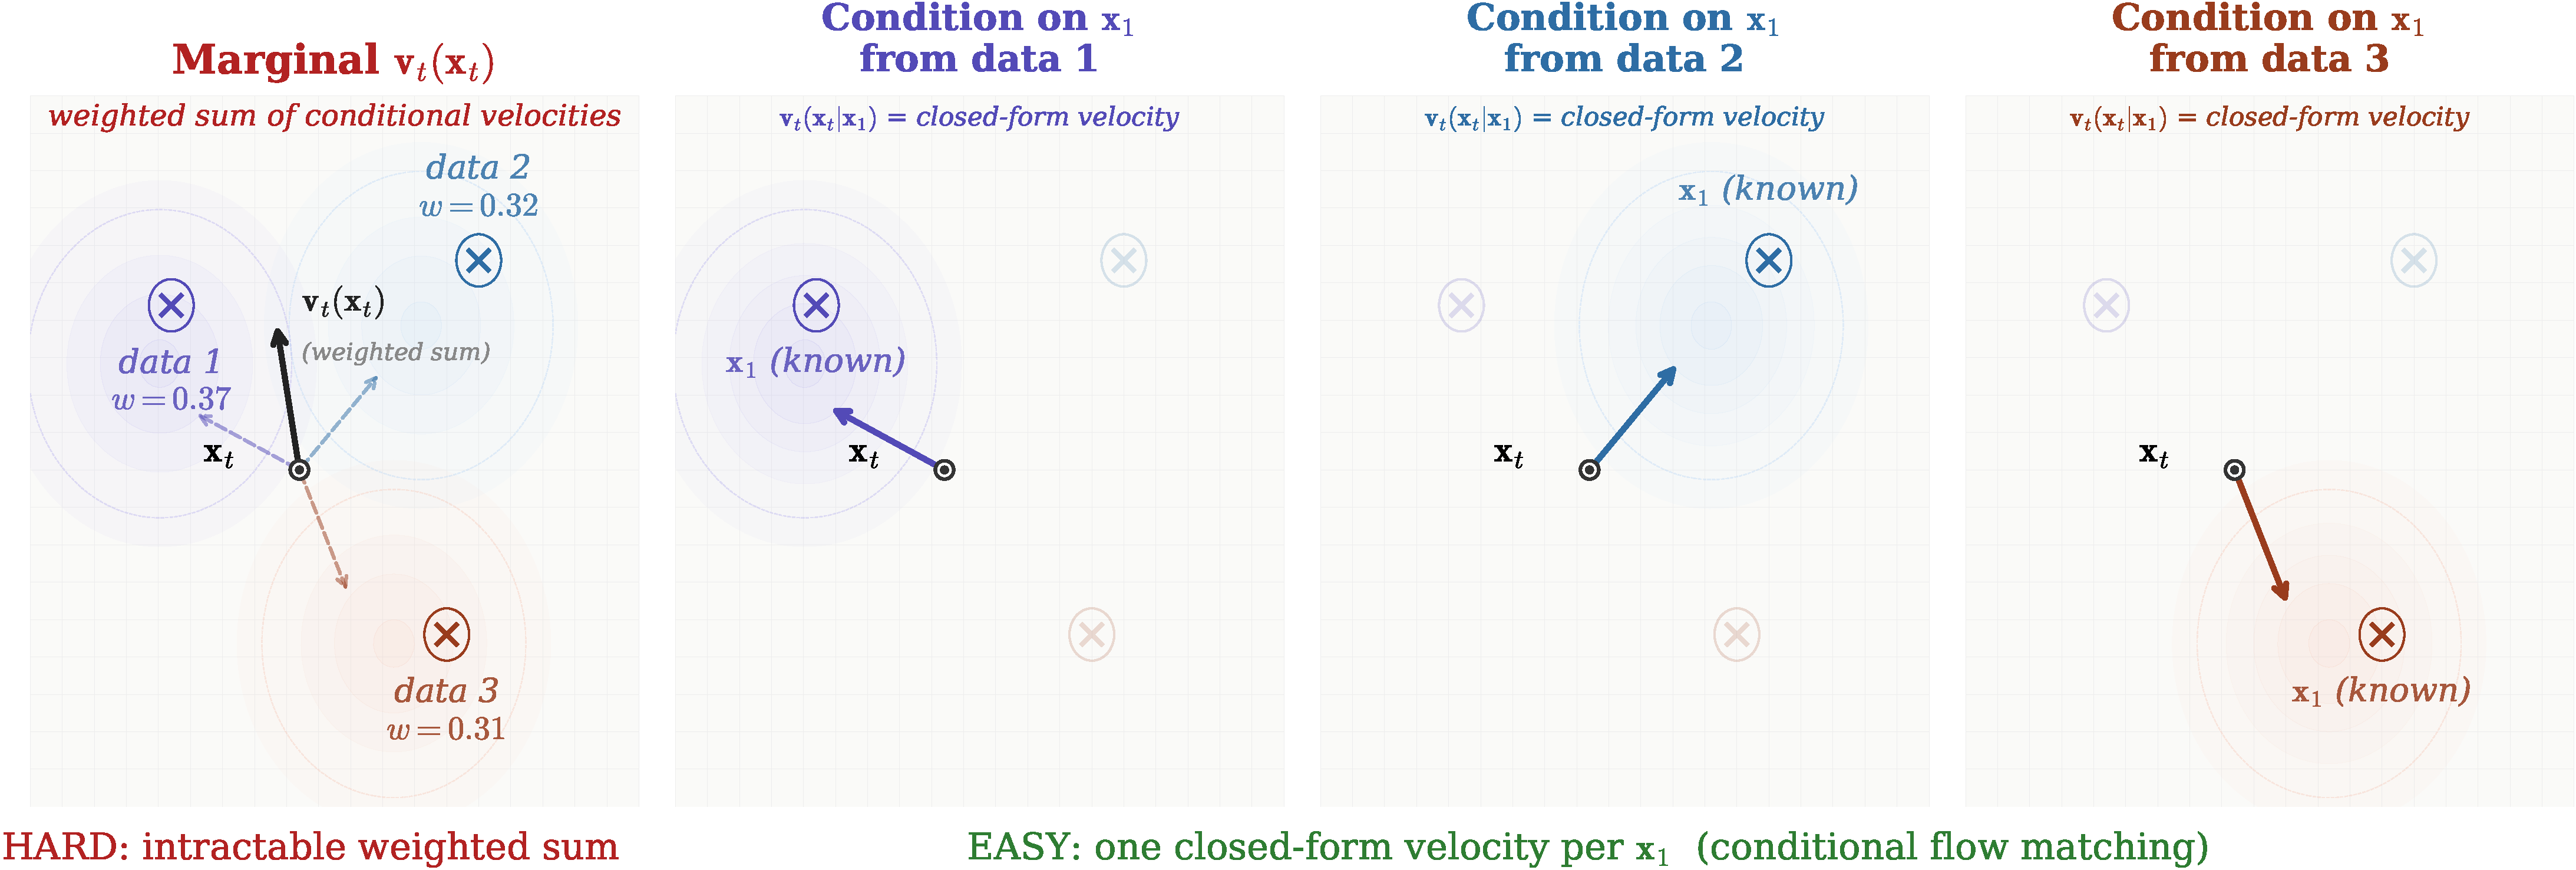
\includegraphics[width=\linewidth]{Images/PartB/flow_matching_conditional.pdf}
    \caption{\textbfs{条件流匹配中的条件技巧（取 $\rvz=\rvx_1\sim p_{\mathrm{tgt}}$）。}
边际速度
$\rvv_t(\rvx_t)=\mathbb{E}_{\rvx_1\sim p(\cdot|\rvx_t)}[\rvv_t(\rvx_t|\rvx_1)]$
（左）是所有目标点 $\rvx_1\sim p_{\mathrm{tgt}}$ 上条件速度的加权平均，权重为每个 $\rvx_1$ 产生当前 $\rvx_t$ 的似然，一般难以计算。
然而对于固定的 $\rvx_1$，条件速度具有闭式
$\rvv_t(\rvx_t|\rvx_1)=b_t'\rvx_1+(a_t'/a_t)(\rvx_t-b_t\rvx_1)$
（Proposition~\ref{closed-form-vf}；右）。
彩色箭头展示这些条件速度，黑色箭头为它们的加权平均。
条件流匹配（Theorem~\ref{thm:fm-cfm}）在这些易处理的条件目标上训练，同时达到与对难处理的边际速度进行回归相同的最优解。
这类似于变分视角中的条件技巧（Theorem~\ref{thm:equiv-marginal-kl}）以及去噪分数匹配中的条件技巧（Theorem~\ref{thm:sm-dsm}）。
\figcredit{由作者在 AI 辅助编程下绘制。}}
    \label{fig:cfm-illustration}
\end{figure}


我们将上述讨论总结如下：
\thmp{$\mathcal{L}_{\mathrm{FM}}$ 与 $\mathcal{L}_{\mathrm{CFM}}$ 的等价性}{fm-cfm}{
下式成立：
\begin{align*}
    \mathcal{L}_{\mathrm{FM}}(\bm{\phi}) = \mathcal{L}_{\mathrm{CFM}}(\bm{\phi}) + C,
\end{align*}
其中 $C$ 是与参数 $\bm{\phi}$ 无关的常数。此外，两个损失的最小化子 $\rvv^*$ 都满足
\[
    \rvv^*(\rvx_t, t) = \rvv_t(\rvx_t), \quad \text{for almost every } \rvx_t \sim p_t,
\]
其中 $\rvv_t(\rvx_t)$ 在 \Cref{eq:marginal-oracle-velocity} 中定义。
}{最小化子的论证与推导与 Proposition~\ref{dsm-minimizer} 中分数匹配情形完全相同的推理。
}

这标志着条件化技巧第三次产生了一个易处理的训练目标，如 \Cref{fig:cfm-illustration} 所示。值得注意的是，变分、基于分数以及基于流的方法都反映了相同的底层原理。



\rmkb{
取 $\pi = p_{\mathrm{data}}$，我们可以应用贝叶斯公式：
\[
p(\rvx_0|\rvx_t) = \frac{p_t(\rvx_t|\rvx_0) p_{\mathrm{data}}(\rvx_0)}{p_t(\rvx_t)},
\]
\Cref{eq:marginal-oracle-velocity} 的一个类似分解在基于分数的模型中出现：
\begin{align*}
    \nabla_{\rvx_t} \log p_t(\rvx_t) 
    &= \mathbb{E}_{\rvx_0 \sim p(\cdot|\rvx_t)} \left[ \nabla_{\rvx_t} \log p_t(\rvx_t|\rvx_0) \right] \\
    &= \mathbb{E}_{\rvx_0 \sim p_{\text{data}}} \left[ \nabla_{\rvx_t} \log p_t(\rvx_t|\rvx_0) \cdot \frac{p_t(\rvx_t|\rvx_0)}{p_t(\rvx_t)} \right],
\end{align*}
它映射了 \Cref{eq:marginal-oracle-velocity} 中的边际化策略。
}

如同 \Cref{subsec:lesson-score} 中那样，其中条件密度 $p_t(\rvx_t|\rvz)$ 和条件速度场 $\rvv_t(\rvx_t|\rvz)$ 必须被显式指定，即 $p_t(\rvx_t|\rvx_0) = \mathcal{N}(\rvx_t; \alpha_t \rvx_0, \sigma_t^2 \rmI)$ 且 $\rvv_t(\rvx_t|\rvx_0) = f(t)\rvx_t - \frac{1}{2}g^2(t)\nabla_{\rvx_t} \log p_t(\rvx_t|\rvx_0)$，一般条件流匹配框架也需要这两个组件。然而，在一般情形下我们尚未构造条件密度 $p_t(\rvx_t|\rvz)$ 或条件速度场 $\rvv_t(\rvx_t|\rvz)$。在 \Cref{sec:instance-fm} 中，我们介绍这些组件的若干常见实例。


\subsection{扩散模型、一般流匹配与 NODE 的比较}\label{subsec:compare-dm-general-fm}


\paragraph{扩散模型与一般流匹配的比较。}
来自 \Cref{subsec:lesson-score} 的见解引出了一个扩展的 FM 框架，它保留了相同的底层原理。为突出它们的相似性，我们在 \Cref{tab:framework_comparison} 中加以总结。


\begin{table}[th]
\caption{扩散模型（或高斯 FM）与一般 FM 框架之间的比较。
此处的一般 FM 框架指的是双侧条件的设定，
其中 $\mathbf{x}_0 \sim p_{\text{src}}$ 与 $\mathbf{x}_1 \sim p_{\text{tgt}}$
独立采样。}
\label{tab:framework_comparison}
\centering
\resizebox{\textwidth}{!}{
\begin{tabular}{lcc}
\toprule
\textbfs{方面} & \textbfs{（基于分数的）扩散模型} & \textbfs{一般 FM} \\
\midrule
源分布 $p_{\mathrm{src}}$ & 高斯先验 & 任意 \\
目标分布 $p_{\mathrm{tgt}}$ & 数据分布 & 任意 \\
隐变量分布 $\pi(\rvz)$ & $p_{\text{data}}$ & 见 \Cref{subsec:fm-instantiations} \\
条件分布 $p_t(\rvx_t|\rvz)$ & $\mathcal{N}(\rvx_t;\alpha_t\rvx_0,\sigma_t^2\rmI)$ & 见 \Cref{subsec:fm-instantiations} \\
边际分布 $p_t(\rvx_t)$ & $\int p_t(\rvx_t|\rvx_0) p_{\mathrm{data}}(\rvx_0) \diff\rvx_0$ & $ \int p_t(\rvx_t|\rvz) \pi(\rvz) \diff\rvz$ \\
条件速度 $\rvv_t(\rvx|\rvz)$  & $f(t) \rvx - \frac{1}{2} g^2(t) \nabla \log p_t(\rvx|\rvx_0)$ & 见 \Cref{subsec:fm-instantiations} \\
边际速度 $\rvv_t(\rvx)$  & $f(t) \rvx - \frac{1}{2} g^2(t) \nabla \log p_t(\rvx)$ & 见 \Cref{eq:marginal-oracle-velocity} \\
学习目标 & $\mathcal{L}_{\text{SM}}=\mathcal{L}_{\text{DSM}}+C$ & $\mathcal{L}_{\mathrm{FM}}=\mathcal{L}_{\mathrm{CFM}}+C$ \\
底层规则 & \multicolumn{2}{c}{Fokker-Planck / 连续性方程} \\
\bottomrule
\end{tabular}
}
\end{table}
我们指出，由于高斯 FM 本质上等价于标准扩散模型（详见 \Cref{ch:all-equivalent}），除非明确说明，否则我们将不对二者加以区分。


\paragraph{与 NODE 的联系。}
FM 可被视为 \Cref{subsec:NODE} 中介绍的 NODE 的一种免仿真替代方案。CNF 在最大似然训练时需要求解 ODE，计算开销巨大，而 FM 通过一个简单的回归损失直接回归到一个预定义的速度场，从而绕过了这一点。关键见解是，当连接源分布与目标分布的边际密度路径固定时，训练期间的精确仿真就变得不必要了。


\subsection{（可选）底层规则}\label{subsec:fm-theory}

\paragraph{连续性方程：质量守恒判据。}
类似于 \Cref{subsec:lesson-score} 中关于 PF-ODE 和 Fokker–Planck 的分析，我们现在给出一个判据，用于验证由 ODE 流诱导的密度路径是否与预定义的路径 $\{p_t\}_{t \in [0,1]}$ 相一致。

考虑在依赖时间的速度场 $\rvv_t$ 下描述粒子流的 ODE：
\[
\frac{\diff \rvx(t)}{\diff t} = \rvv_t\left(\rvx(t)\right).
\]
如同 \Cref{eq:pushforward-ode} 中那样，该 ODE 对任意 $s,t \in [0,1]$ 定义了一个流映射
$\bm{\Psi}_{s\to t}(\rvx_0)$，特别地它将 $0$ 时刻的初始点
$\rvx_0 \sim p_{\mathrm{src}}$ 携带至其在 $t$ 时刻的状态。
$t$ 时刻诱导的分布由前推给出：
\begin{align}\label{eq:ode-pushforward}
    p_t^{\mathrm{fwd}}(\rvx)
    = \int \delta \left(\rvx - \bm{\Psi}_{0\to t}(\rvx_0)\right)
      p_{\mathrm{src}}(\rvx_0) \mathrm{d}\rvx_0=: \bm{\Psi}_{0\to t}\# p_{\mathrm{src}},
\end{align}
因此当 $\rvx_0 \sim p_{\mathrm{src}}$ 时，有 $\bm{\Psi}_{0\to t}(\rvx_0) \sim p_t^{\mathrm{fwd}}$。
类似地，可以借助 $\bm{\Psi}_{1\to 0}(\rvx_1)$ 从 $\rvx_1 \sim p_{\mathrm{tgt}}$
反向传输到 $p_{\mathrm{src}}$。




假设我们给定了一条预定义的密度路径 $\{p_t\}_{t \in [0,1]}$，并构造一个速度场 $\{\rvv_t\}_{t \in [0,1]}$ 来定义粒子流。这自然引出了一个问题：

\begin{question}
    在什么条件下，流诱导的密度 $p_t^{\mathrm{fwd}}$ 在所有 $t \in [0,1]$ 上恰好匹配目标密度 $p_t$？
\end{question}
一旦这两个密度演化相一致，我们就可以通过求解 ODE 利用 ODE 流在 $p_{\mathrm{src}}$ 和 $p_{\mathrm{tgt}}$ 之间灵活地传输样本。

如同 \Cref{eq:p_t-fwd-rev} 中那样，验证这种一致性的一个有原则的方法是借助 \emph{连续性方程}，它刻画了时间演化密度中的质量守恒：

\thmp{质量守恒判据}{continuity-mass}{
流诱导的密度 $p_t^{\mathrm{fwd}}$ 在所有 $t \in [0,1]$ 上等于预定义路径 $p_t$；即
\[
p_t^{\mathrm{fwd}} = p_t, \quad \text{for all } t \in [0,1],
\]
当且仅当对 $(p_t, \rvv_t)$ 满足连续性方程：
\[
\partial_t p_t(\rvx) + \nabla_\rvx \cdot (p_t(\rvx) \rvv_t(\rvx)) = 0,
\]
对所有 $t\in[0,1]$ 和 $\rvx$ 成立。
}{\Cref{app-sec:mass-conservation} 中给出了概念性推导，更严格的处理可参见 \citep{villani2008optimal}（参见其中的“Mass Conservation Formula”）。}

\paragraph{从条件路径到边际路径。}正如 \Cref{subsec:fm-framework} 所见，我们先定义一个条件概率路径 $p_t(\cdot| \rvz)$ 和相应的条件速度场 $\rvv_t(\cdot| \rvz)$。然后我们通过下式构造边际速度场：
\[
    \rvv_t(\rvx) 
    = \int \rvv_t(\rvx| \rvz) \frac{p_t(\rvx| \rvz) \pi(\rvz)}{p_t(\rvx)}   \diff \rvz,
\]
如 \Cref{eq:marginal-oracle-velocity} 所述。然而，我们仍需确保所得边际速度 $\rvv_t$ 诱导的 ODE 流的密度路径与预定义的 $p_t$ 相一致。幸运的是，这一验证可以完全在条件层面进行：如果每个条件速度场 $\rvv_t(\cdot| \rvz)$ 诱导的条件密度路径为 $p_t(\cdot| \rvz)$，那么所得的边际速度 $\rvv_t$ 也会诱导正确的边际路径。形式化地，这表述如下：

\proppp{边际速度场生成给定边际密度}{marginal-vf}{
若条件速度场 $\rvv_t(\cdot|\rvz)$ 诱导的条件密度路径与 $p_t(\cdot|\rvz)$ 相匹配（从 $p_0(\cdot|\rvz)$ 出发），则 \Cref{eq:marginal-oracle-velocity} 中定义的边际速度场 $\rvv_t(\cdot)$ 诱导的边际密度路径与 $p_t(\cdot)$ 相一致，从 $p_0(\cdot)$ 出发。
}{
该结果通过验证对 $(p_t, \rvv_t)$ 满足连续性方程得到。我们以反过来的方式给出论证，以提供关于为何边际化后的速度场取 \Cref{eq:marginal-oracle-velocity} 这一形式的直观理解。
由于条件速度场 $\rvv_t(\cdot|\rvz)$ 对 $\rvz \sim \pi$ 诱导的密度路径与条件密度 $p_t(\cdot|\rvz)$ 相匹配，连续性方程对每个条件对成立：
\begin{align}\label{eq:continuity_conditional_pt}
    \frac{\diff}{\diff t} p_t(\rvx|\rvz) =- \nabla_\rvx \cdot \big(\rvv_t(\rvx|\rvz) p_t(\rvx|\rvz)\big).
\end{align}
我们希望找到一个速度场 ${\color{orange}\rvv_t(\cdot)}$，其诱导的密度与边际密度 $p_t$ 相一致，即满足
\begin{align}\label{eq:p_t_continuity}
    \frac{\diff}{\diff t} p_t(\rvx) =- \nabla_\rvx \cdot \big({\color{orange}\rvv_t(\rvx)} p_t(\rvx)\big).
\end{align}
从 \Cref{eq:p_t} 中 $p_t$ 的定义出发，
\begin{align*}
  \frac{\diff}{\diff t} p_t(\rvx) &=\int \frac{\diff}{\diff t} p_t(\rvx_t|\rvz)\pi(\rvz)\diff \rvz \nonumber\\
  &=  - \int \nabla_\rvx \cdot\Big(  \rvv_t(\rvx|\rvz) p_t(\rvx | \rvz)  \Big)\pi(\rvz) \diff \rvz \quad \nonumber \\
  &=  -\nabla_\rvx \cdot \Big( \int  \rvv_t(\rvx|\rvz) p_t(\rvx | \rvz) 
 \pi(\rvz) \diff \rvz\Big), \nonumber  
\end{align*}
其中第二个等号由应用 \Cref{eq:continuity_conditional_pt} 得到。将其与 \Cref{eq:p_t_continuity} 的右边相比较可知，至多差一个无散项，
\[
    {\color{orange}\rvv_t(\rvx)} p_t(\rvx) = \int \rvv_t(\rvx|\rvz) p_t(\rvx|\rvz) \pi(\rvz) \diff \rvz.
\]
因此我们可以定义
\[
    {\color{orange}\rvv_t(\rvx)} := \int \rvv_t(\rvx|\rvz) \frac{p_t(\rvx|\rvz)}{p_t(\rvx)} \pi(\rvz) \diff \rvz,
\]
这正是 \Cref{eq:marginal-oracle-velocity} 中的形式。
本定理的证明本质上沿着与此论证相反的方向进行。
}

这一联系使我们可以将构造潜在的不可处理的边际速度场，归约为定义更简单的条件速度场 $\rvv_t(\cdot| \rvz)$，而后者按构造更易于处理。




\newpage

\section{在分布之间构造概率路径与速度}\label{sec:instance-fm}

流匹配的本质在于将一个源分布逐步变换为目标分布。为引导这一变换，需要两个关键要素：\emph{概率路径} $p_{t}$，它在每个时刻 $t$ 提供演化分布的一个快照；以及 \emph{速度场} $\rvv_{t}$，它描述单个粒子如何沿路径移动。这两个对象并非独立；它们通过连续性方程相联系，后者保证粒子动力学与分布的演化相一致。因此，学习任务归结为寻找一个忠实驱动该过程的速度场 $\rvv_t$。然而困难在于，对于一般且复杂的分布，真实的边际速度 $\rvv_t$ 是未知的，留下一个无法直接访问的不可处理目标。

条件流匹配的核心思想是通过构造一个人为但易处理的过程，来应对真实边际速度的不可处理性。为此，我们引入一个条件变量 $\rvz$，并设计一个条件速度 $\rvv_t(\rvx_t|\rvz)$ 和/或一个条件路径 $p_t(\rvx_t|\rvz)$，它们被刻意选得简单。

 因为这些条件对象具有已知的闭式形式，它们可作为模型回归的替代目标。只要满足两个实际要求，这就导出了一个有效的训练损失 $\mathcal{L}_{\mathrm{CFM}}$：（i）我们能从 $p_t(\cdot|\rvz)$ 中高效采样；（ii）相应的速度 $\rvv_t(\cdot|\rvz)$ 具有闭式表达。


我们应当如何设计一个良好行为的条件过程？为获得启发，我们转向那个已被完全理解的情况：高斯到高斯的桥（\Cref{subsec:special-fm-instantiations}）。该示例突出了两种自然的设计策略：在每个时刻 $t$ 采用高斯概率路径，或指定一个仿射速度场，两者在解析上都是易处理的。

在此见解指引下，我们以两种互补的视角将其推广到一般端点分布（另见 \Cref{subsec:cov-continuity-eq}），用于构造条件路径和速度：
\begin{itemize}
    \item \textbfs{条件概率路径优先（欧拉视角）。}先从一个条件概率路径 $p_t(\cdot|\rvz)$ 出发，再推导相应的条件速度场。
    \item \textbfs{条件流优先（拉格朗日视角）。}先从一个条件流 $\bPsi_{0\to t}(\cdot|\rvz)$（通常是仿射的）出发，通过对沿轨迹关于时间求导来推导条件速度场。
\end{itemize}


在 \Cref{subsec:fm-instantiations} 中，我们详细阐述第一种方法，它表明其与 \Cref{subsec:lesson-score} 中讨论的扩散模型构造有紧密类比；而在 \Cref{subsec:prob-path-flow} 中我们给出第二种方法。这两种视角共同提供了一个定义 $p_t(\rvx_t| \rvz)$ 与 $\rvv_t(\rvx_t| \rvz)$ 的实用框架，能够实现免仿真训练以及在任意源分布和目标分布之间构造流。





\subsection{关键特例：高斯到高斯桥中的边际 $p_t(\rvx_t)$ 与速度 $\rvv_t(\rvx_t)$}\label{subsec:special-fm-instantiations}

我们从高斯端点的情形开始，此时我们可以解析地计算边际密度 $p_t(\rvx_t)$ 和速度场 $\rvv_t(\rvx_t)$。这为一般情形下条件密度 $p_t(\rvx_t |\rvz_t)$ 和速度场 $\rvv_t(\rvx_t |\rvz_t)$ 的构造提供了一个模板。



当源分布和目标分布 $p_{\text{src}}$ 与 $p_{\text{tgt}}$ 都为高斯时，速度场 $\rvv_t(\cdot)$ 具有闭式表达。我们考虑如下的插值边际密度路径：
\begin{align}\label{eq:gaussian-density-path}
    p_t(\rvx_t) = \mathcal{N}\left(\rvx_t; \bm{\mu}(t), \sigma^2(t) \rmI\right),
\end{align}
具有随时间变化的均值 $\bm{\mu}(t)$ 和方差 $\sigma^2(t)>0$。两个端点由下式给出
\[
p_{\text{src}} = p_0 =  \mathcal{N}\left(\rvx; \bm{\mu}(0), \sigma^2(0) \rmI\right), \quad
p_{\text{tgt}} = p_1 =  \mathcal{N}\left(\rvx; \bm{\mu}(1), \sigma^2(1) \rmI\right),
\]
于是路径 $\{p_t\}_{t \in [0,1]}$ 将这些分布连接起来。

对于给定路径 $\{p_t\}_{t \in [0,1]}$，确实存在许多速度场都能诱导一个 ODE 流 $\bm{\Psi}_{0\to t}(\rvx)$ 使得 $\rvx \sim p_0$ 蕴含 $\bm{\Psi}_{0\to t}(\rvx) \sim p_t$。对于这条高斯路径，一个特别简单的实现为\footnote{在 \citep{lipman2022flow} 中，作者考虑 $\bm{\Psi}_{0\to t}(\rvx) = \bm{\mu}(t) + \sigma(t)\rvx$，它要求对 $\bm{\mu}(t)$ 与 $\sigma(t)$ 施加约束以保证边界条件。我们采用一个等价的归一化形式，可避免此类约束。}：
\begin{align}\label{eq:gaussian-sol-map}
    \bm{\Psi}_{0\to t}(\rvx) := \bm{\mu}(t) + \sigma(t) \left( \frac{\rvx - \bm{\mu}(0)}{\sigma(0)} \right).
\end{align}

对于定义的高斯路径 $p_t$（对所有 $t$ 均为高斯），诱导 \Cref{eq:gaussian-sol-map} 中 ODE 流的速度场 $\rvv_t(\cdot)$ 被唯一地以解析形式刻画如下~\citep{lipman2022flow}：

\proppp{高斯密度路径的闭式速度场}{closed-form-vf}{
设 $p_t$ 为 \Cref{eq:gaussian-density-path} 中的高斯路径。则产生 ODE 流 \Cref{eq:gaussian-sol-map} 的速度场 $\rvv_t(\cdot)$ 对于所定义的 $\bPsi_{0\to t}$ 是唯一的，并具有如下闭式表达：
\begin{equation*}
    \rvv_t(\rvx) = \frac{\sigma'(t)}{\sigma(t)} \left( \rvx - \bm{\mu}(t) \right) + \bm{\mu}'(t).
\end{equation*}
}{考虑具有初值 $\rvy$ 的 ODE：
\[
    \frac{\diff}{\diff t} \bm{\Psi}_{0\to t}(\rvy) = \rvv_t(\bm{\Psi}_{0\to t}(\rvy)).
\]
由于 $\bm{\Psi}_{0\to t}$ 可逆（因 $\sigma(t)>0$），我们可令 $\rvx = \bm{\Psi}_{0\to t}(\rvy)$ 且 $\rvy = \bm{\Psi}_{0\to t}^{-1}(\rvx) = \bm{\Psi}_{t\to 0}(\rvx)$ 得到
\[
    \bm{\Psi}_{0\to t}'\big(\bm{\Psi}_{0\to t}^{-1}(\rvx)\big) = \rvv_t(\rvx).
\]
对 \Cref{eq:gaussian-sol-map} 关于 $t$ 求导给出
\begin{equation*}
    \bm{\Psi}_{0\to t}'(\rvx) = \bm{\mu}'(t) + \sigma'(t) \left( \frac{\rvx - \bm{\mu}(0)}{\sigma(0)} \right).
\end{equation*}
解出 $\rvy = \bm{\Psi}_{0\to t}^{-1}(\rvx)$ 得
\[
    \rvy = \bm{\mu}(0) + \sigma(0) \left( \frac{\rvx - \bm{\mu}(t)}{\sigma(t)} \right).
\]
将其代入 $\bm{\Psi}_{0\to t}'(\rvx)$ 得
\[
    \rvv_t(\rvx) = \frac{\sigma'(t)}{\sigma(t)} \left( \rvx - \bm{\mu}(t) \right) + \bm{\mu}'(t),
\]
如所断言。
}
我们注意到，对于一个固定的流映射 $\bPsi_{0\to t}$（流优先视角），速度被唯一地由下式确定：
\[
\rvv_t  =  \partial_t \bPsi_{0\to t} \circ \bPsi_{0\to t}^{-1}.
\]
在此构造下，对 $(p_t,\rvv_t)$ 自动满足连续性方程。
相比之下，对于一个给定的密度路径 $t\mapsto p_t$ 而不固定 $\bPsi_{0\to t}$（概率路径优先视角），
速度场并不是唯一的。

这一区别恰好刻画了流优先视角与概率路径优先视角之间的差异。



这一闭式刻画在对隐变量 $\rvz$ 加条件化时仍然成立。
下面我们将这一见解加以推广，构造一般边际设定下的条件高斯路径 $p_t(\cdot|\rvz)$
并推导相应的条件速度场 $\rvv_t(\cdot|\rvz)$。




\subsection{$\rvv_t(\cdot|\rvz)$ 与 $p_t(\cdot|\rvz)$ 的条件概率路径优先构造}\label{subsec:fm-instantiations}


\begin{figure}[th!]
    \centering
    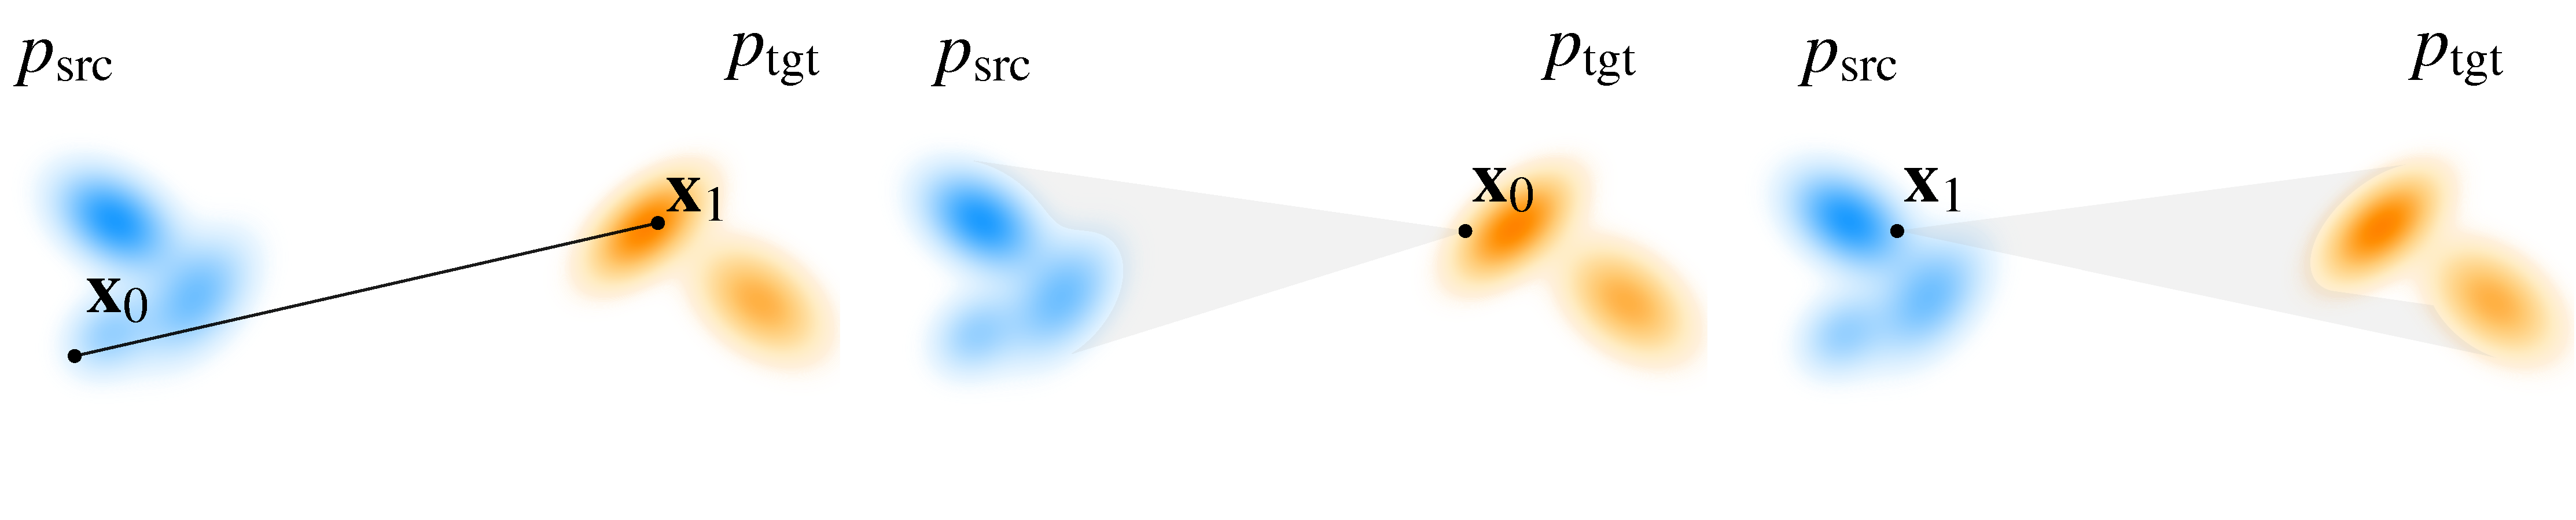
\includegraphics[width=\linewidth]{Images/PartB/triptych_gray_cones_final.pdf}
    \caption{\textbfs{两类常见条件概率路径的示意图}。包括：
（i）\emph{双侧}，以 $\rvx_0 \sim p_{\text{tgt}}$ 与 $\rvx_1 \sim p_{\text{src}}$ 为条件且端点为一般分布；
（ii）\emph{单侧}，以 $\rvx_0 \sim p_{\text{tgt}}$ 或 $\rvx_1 \sim p_{\text{src}}$ 之一为条件。
\figcredit{由作者绘制。}}
    \label{fig:conditional-path}
\end{figure}

我们的目标是先构造一个条件密度路径 $p_t(\cdot|\rvz)$，再推导其对应的条件速度场 $\rvv_t(\cdot|\rvz)$（通过 Proposition~\ref{closed-form-vf}），所基于的是关于 $\pi(\rvz)$ 的条件化。
依据 $\rvz$ 的选取方式，存在两种自然情形：
（i）双侧条件 $\rvz=(\rvx_0,\rvx_1)$，或
（ii）单侧条件 $\rvz=\rvx_0$ 或 $\rvx_1$。
在两种情形下，构造都必须匹配边界分布：
\begin{align*}
   p_{\mathrm{src}}(\rvx_0) = \int p_0(\rvx_0|\rvz) \pi(\rvz)\diff\rvz, \quad
   p_{\mathrm{tgt}}(\rvx_1) = \int p_1(\rvx_1|\rvz) \pi(\rvz) \diff\rvz.
\end{align*}
由于一旦指定了具体构造后验证这些约束非常直接，我们在此不再强调验证步骤。



\paragraph{I. 双侧 $\rvz = (\rvx_0, \rvx_1)$ —— “光束式”路径。}
    \subparagraph{$\pi(\rvz)$ 的选择。}考虑 $\mathbb{R}^D$ 上的一般分布 $p_{\mathrm{src}}$ 和 $p_{\mathrm{tgt}}$。令 $\rvz = (\rvx_0, \rvx_1)$，其中 $\rvx_0 \sim p_{\mathrm{src}}$ 与 $\rvx_1 \sim p_{\mathrm{tgt}}$ 相互独立，即
    \[
    \pi(\rvz) = p_{\mathrm{src}}(\rvx_0)  p_{\mathrm{tgt}}(\rvx_1).
    \]
    \subparagraph{条件路径 $p_t(\cdot|\rvz)$ 的选择。}用固定方差 $\sigma > 0$ 的线性插值定义条件路径：
    \[
    p_t(\rvx_t | \rvz = (\rvx_0, \rvx_1)) = \mathcal{N}(\rvx_t; a_t\rvx_0 + b_t\rvx_1,  \sigma^2 \rmI),
    \]
    其中 $a_t$ 和 $b_t$ 是依赖时间的函数，满足  $a_0 = 1,  b_0 = 0$ 和 $a_1 = 0,  b_1 = 1$。\citep{lipman2022flow,liu2022rectified} 建议的一种选取为 $a_t = 1-t$，$b_t = t$。在确定性情形 $\sigma = 0$ 下，我们得到
\[
p_t(\rvx_t |\rvz) = \delta \big(\rvx_t - [a_t\rvx_0 + b_t\rvx_1]\big),
\]
它描述了一条从 $\rvx_0$ 到 $\rvx_1$ 的确定性插值路径。
    \subparagraph{导出的条件速度 $\rvv_t(\cdot|\rvz)$。}由 Proposition~\ref{closed-form-vf}，条件速度为
    \[
    \rvv_t(\rvx | \rvz) = a'_t\rvx_0 + b'_t\rvx_1.
    \]
    \subparagraph{CFM 损失。}当 $\sigma=0$ 使得 $\rvx_t = a_t\rvx_0 + b_t\rvx_1$ 时，CFM 损失简化为
    \[
    \mathcal{L}_{\mathrm{CFM}} = \mathbb{E}_{t, \rvx_0\sim p_{\text{src}}, \rvx_1\sim p_{\text{tgt}}} \left\| \rvv_{\bm{\phi}}(\rvx_t, t) - \left(a'_t\rvx_0 + b'_t\rvx_1\right) \right\|^2.
    \]
由 \Cref{eq:marginal-oracle-velocity,eq:minimum_velocity}，最优速度场为
\[
\rvv^*(\rvx_t, t) = \mathbb{E} \left[ \rvx_t'|\rvx_t \right] = \mathbb{E} \left[ a'_t\rvx_0 + b'_t\rvx_1|\rvx_t \right].
\]
这里期望是在 $p(\mathbf{x}_0, \mathbf{x}_1|\mathbf{x}_t)$ 上取的，即在 $t$ 时刻能产生观测插值 $\mathbf{x}_t = a_t\mathbf{x}_0 + b_t\mathbf{x}_1$ 的所有源-目标对 $(\mathbf{x}_0, \mathbf{x}_1)$ 上的条件分布。



\paragraph{II. 单侧 $\rvz = \rvx_0$ 或 $\rvx_1$ —— “聚光式”路径。}
我们在单侧设定下阐述条件概率路径优先的构造，考虑标准的生成设定，即 $p_{\mathrm{src}}=\mathcal N(\bm 0,\rmI)$ 且 $p_{\mathrm{tgt}}=p_{\mathrm{data}}$。
关键的是，这一高斯源并非额外的假设，而是下面定义的条件路径的直接结果。
对任意端点更一般的处理见 \Cref{subsec:prob-path-flow}。

\subparagraph{$\pi(\rvz)$ 的选择。}
我们取 $\rvz=\rvx_1$，$\pi(\rvz)=p_{\mathrm{data}}(\rvx_1)$（$\rvz=\rvx_0\sim p_{\mathrm{prior}}$ 的情形可类似地处理）。

\subparagraph{条件路径 $p_t(\cdot|\rvz)$ 的选择。}
对固定的 $\rvx_1\sim p_{\mathrm{data}}$，定义
\[
p_t(\rvx_t|\rvz=\rvx_1)=\mathcal N \big(\rvx_t; b_t \rvx_1, a_t^2 \rmI\big),
\]
其中 $ a_0=1, b_0=0, a_1=0, b_1=1$（通常解释为极限）。
在边界处，
\[
p_0(\cdot|\rvz=\rvx_1)=\mathcal N(\cdot; \bm 0,\rmI),\qquad
p_1(\cdot|\rvz=\rvx_1)=\delta(\cdot - \rvx_1).
\]
对 $\rvx_1$ 取边际得到 $\{p_t\}_{t\in[0,1]}$，其中
$p_0=\mathcal N(\bm 0,\rmI)$（与 $p_{\mathrm{data}}$ 无关）且 $p_1=p_{\mathrm{data}}$。

\subparagraph{导出的条件速度 $\rvv_t(\cdot|\rvz)$。}
对于 $t\in(0,1)$ 且 $b_t>0$，将 Proposition~\ref{closed-form-vf} 应用于条件高斯路径得到
\[
\mathbf v_t(\rvx|\rvx_1)
= b_t' \rvx_1 + \frac{a_t'}{a_t} \big(\rvx - b_t \rvx_1\big).
\]

\subparagraph{单侧 CFM 目标。}
取 $t\sim\mathcal U(0,1)$（或任意固定的采样分布）且 $\rvx_1\sim p_{\mathrm{data}}$，CFM 损失变为
\begin{align}\label{eq:one-sided-cfm}
    \mathcal L_{\mathrm{CFM}}
=\E_{t,\rvx_1} \E_{\rvx_t\sim p_t(\cdot|\rvx_1)}
\Big\|\mathbf v_\phi(\rvx_t,t)-
\Big[b_t'\rvx_1+\tfrac{a_t'}{a_t}\big(\rvx_t-b_t\rvx_1\big)\Big]\Big\|_2^2.
\end{align}
由 MSE 最优性，唯一的最小化子是边际速度场
\[
\mathbf v^*(\rvx,t)
= \E \left[\mathbf v_t(\rvx|\rvx_1) |dle|  \rvx_t=\rvx\right]
= \E \left[a_t'\rvx_0+b_t'\rvx_1 |dle|  \rvx_t=\rvx\right].
\]

\subparagraph{与双侧目标的等价性。}
对成对样本 $(\rvx_0,\rvx_1)$ 且 $\rvx_t=a_t\rvx_0+b_t\rvx_1$，
\[
\mathbf v_t(\rvx_t|\rvx_1)
= b_t'\rvx_1 + \tfrac{a_t'}{a_t}\big(\rvx_t-b_t\rvx_1\big)
= a_t'\rvx_0 + b_t'\rvx_1.
\]
Thus the one-sided loss regresses to the \emph{conditional expectation} of the two-sided target given $\rvx_t$:
\[
\mathbf v^*(\rvx,t)=\E \big[a_t'\rvx_0 + b_t'\rvx_1 | \rvx_t=\rvx\big],
\]
so the one-sided and two-sided CFM objectives share the same minimizer.


\paragraph{Gaussian FM = Diffusion Model.}
We use the FM convention where $t=0$ denotes the source/prior and $t=1$ denotes the target/data:
\[
p_{\mathrm{src}}=p_{\mathrm{prior}},\qquad p_{\mathrm{tgt}}=p_{\mathrm{data}}.
\]
By contrast, diffusion models typically index time from data to noise (i.e., $t=0$ is data and $t=1$ is prior). 
Here, we adopt the FM convention indexing in the main discussion. For comparison, however, the VE and VP entries in \Cref{tb:interpolant_instances} are summarized in their usual diffusion-time indexing, where $t=0$ corresponds to data and $t=1$ to prior/noise.
If further $p_{\mathrm{src}}=\mathcal N(\bm 0,\rmI)$, then for fixed condition $\rvx_1\sim p_{\mathrm{data}}$, 
the conditional path $p_t(\cdot |\rvx_1)$ is naturally chosen to be Gaussian, 
while the target distribution $p_{\mathrm{tgt}}$ itself need not be Gaussian. Some literature usually refer to this setting as \emph{Gaussian FM}.



Choosing $a_t = 1-t$ and $b_t = t$ (equivalently, $\alpha_t = t$ and $\sigma_t = 1-t$ under the relabeling $a_t:=\sigma_t$, $b_t:=\alpha_t$ in diffusion model) recovers the familiar FM/RF schedule~\citep{lipman2022flow,liu2022rectified}.


\begin{table}[th]
\caption{Summary of different interpolants written as 
  $\rvx_t = a_t \rvx_0 + b_t \rvx_1$, where 
  $\rvx_0 \sim p_{\mathrm{src}}=p_{\mathrm{prior}}$ and 
  $\rvx_1 \sim p_{\mathrm{tgt}}=p_{\mathrm{data}}$. 
  The FM/RF and trigonometric columns use the FM convention ($t=0$ source, $t=1$ target). 
  For comparison, the VE/VP columns retain their usual diffusion-time indexing ($t=0$ data, $t=1$ prior/noise), with coefficient names relabeled as $a_t:=\sigma_t$ and $b_t:=\alpha_t$.}
  \small
  \centering
  \resizebox{\textwidth}{!}{
  \begin{tabular}{lcccc}
     \toprule
         & \textbfs{VE} & \textbfs{VP} & \textbfs{FM/RF} & \textbfs{Trig.}~\citep{albergo2023stochastic} \\
    \midrule
     $a_t$ (prior coeff.) 
       & $a_t$ 
       & $\sqrt{1-b_t^2}$ 
       & $1-t$ 
       & $\cos \bigl(\tfrac{\pi}{2}t\bigr)$ \\
     $b_t$ (data coeff.) 
       & $1$ 
       & $b_t$ 
       & $t$ 
       & $\sin \bigl(\tfrac{\pi}{2}t\bigr)$ \\
    \midrule
     $a_0$ & $0$ & $0$ & $1$ & $1$ \\
     $b_0$ & $1$ & $1$ & $0$ & $0$ \\
     $a_1$ & $a_1$ & $1$ & $0$ & $0$ \\
     $b_1$ & $1$ & $0$ & $1$ & $1$ \\
    \midrule
     $p_{\text{prior}}$ 
       & $\mathcal{N}(\bm{0},a_1^2\rmI)$ 
       & $\mathcal{N}(\bm{0},\rmI)$ 
       & $\mathcal{N}(\bm{0},\rmI)$ 
       & $\mathcal{N}(\bm{0},\rmI)$ \\
     \bottomrule
  \end{tabular}}
  \label{tb:interpolant_instances}
\end{table}



In the Gaussian FM setting, both the beam-like and spotlight-like conditional paths lead to training objectives that are  similar to the standard diffusion losses. As we will elaborate in \Cref{ch:all-equivalent}, Gaussian FM can in fact be equivalently interpreted as a diffusion model trained to predict the \emph{velocity}, under the linear schedule $a_t = 1-t$ and $b_t = t$. This perspective highlights that flow matching and diffusion are not fundamentally different, but rather two equivalent formulations that can be transformed into one another. The Gaussian FM objective is particularly appealing in practice: its loss function ($\E_{t,\rvx_t} \left[\norm{\rvv_\bphi(\rvx_t, t) - (\rvx_1 - \rvx_0)}_2^2\right]$) is simple, and it has been shown to achieve competitive performance at scale~\citep{esser2024scaling}. 




\subsection{Conditional Flow-First Construction of $\rvv_t(\cdot|\rvz)$ and $p_t(\cdot|\rvz)$}\label{subsec:prob-path-flow}

We treat the general case where the endpoints $p_{\mathrm{src}}$ (at $t=0$) and $p_{\mathrm{tgt}}$ (at $t=1$) are arbitrary. 
Our goal is to design, directly in trajectory space, a conditional flow that transports samples from $p_{\mathrm{src}}$ to $p_{\mathrm{tgt}}$ and yields a closed-form $\rvv_t(\rvx_t|\rvz)$ usable as a regression target.

\paragraph{Motivation.}
Instead of first designing conditional density path, we may directly specify a conditional flow map $\bPsi_{0\to t}(\cdot;\rvz)$ that moves samples along trajectories. This has two practical advantages: (i) it immediately yields a regression target for training via a time derivative along trajectories; (ii) on geometry-structured spaces (Riemannian manifolds, Lie groups, or constrained submanifolds), it is often natural to construct the conditional flow map 
$\bPsi_{0\to t}$ directly from the geometry (e.g., geodesics, exponential maps, or premetrics)~\citep{lipman2024flow} which yields analytic, simulation-free target velocities for training.


\paragraph{Conditional Affine Flow (Link to Proposition~\ref{closed-form-vf}).}
We fix a conditioning variable $\rvz\sim\pi$ (e.g., $\rvz=\rvx_1\sim p_{\mathrm{tgt}}$ in one-sided “spotlight’’ training) and push forward $\rvx_0\sim p_{\mathrm{src}}$ through the time-varying \emph{conditional affine flow} 
\[
\bPsi_{0\to t}(\rvx_0;\rvz) := \bm\mu_t(\rvz) + \rmA_t(\rvz) \rvx_0,\qquad t\in[0,1],
\]
where $\bm\mu_t(\rvz)\in\R^D$ and $\rmA_t(\rvz)\in\R^{D\times D}$ is invertible for $t\in(0,1)$. The boundary 
$\rmA_0(\rvz)=\rmI,\ \bm\mu_0(\rvz)=\mathbf 0$ recovers $p_{\mathrm{src}}$ at $t=0$. It is standard to interpret boundary when $t\to1$ as a limit (the terminal map may concentrate mass on a lower-dimensional set or a point)\footnote{Allowing $\rmA_1(\rvz)$ to be singular (e.g., $\mathbf 0$) is compatible with invertibility on $(0,1)$ and causes the path to contract onto the prescribed endpoint at $t=1$.}. 


\subparagraph{Induced Conditional Path $p_t(\cdot|\rvz)$.}
The construction defines
\[
p_t(\cdot|\rvz) = \bigl(\bPsi_{0\to t}( \cdot ;\rvz)\bigr)_{\#} p_{\mathrm{src}},
\qquad
p_t(\cdot)  =  \int p_t(\cdot|\rvz)\pi(\rvz)\diff\rvz.
\]
What ultimately matters in $\mathcal{L}_{\mathrm{CFM}}$ is how to sample from it:  
first draw $\rvz \sim \pi$, then draw $\rvx_0 \sim p_{\mathrm{src}}$, and finally set
\[
\rvx_t = \bm\mu_t(\rvz) + \rmA_t(\rvz)\rvx_0.
\]


We remark that when $\bPsi_{0\to t}$ is affine in $\rvx_0$, then $p_t( \cdot | \rvz)$ is Gaussian 
if and only if $p_{\mathrm{src}}$ is Gaussian. 
In particular, for arbitrary (non-Gaussian) $p_{\mathrm{src}}$, an affine flow yields a
generally non-Gaussian $p_t(\cdot|\rvz)$.


\subparagraph{Derived Conditional Velocity $\rvv_t(\cdot|\rvz)$.} The conditional velocity $\rvv_t(\cdot|\rvz)$ is obtained by $t$-differentiating the conditional flow map $\bPsi_{0\to t}$. Following the derivation in Proposition~\ref{closed-form-vf}, consider the \emph{conditional} ODE defined by the flow map $\bPsi_{0\to t}(\rvy;\rvz)$ with initial condition $\rvy$, where the goal is to identify the corresponding conditional velocity field $\rvv_t(\cdot|\rvz)$:
\[
\frac{\diff}{\diff t} \bPsi_{0\to t}(\rvy;\rvz)
= \rvv_t \Big(\underbrace{\bPsi_{0\to t}(\rvy;\rvz)}_{\rvx} \Big| \rvz\Big).
\]
Since $\bPsi_{0\to t}(\cdot;\rvz)$ is invertible for $t\in(0,1)$, we may express $\rvy$ in terms of the current state $\rvx:=\bPsi_{0\to t}(\rvy;\rvz)$ as $\rvy=\bPsi_{0\to t}^{-1}(\rvx;\rvz)=\bPsi_{t\to 0}(\rvx;\rvz)$. Substituting this into the ODE yields the following construction of the conditional velocity field:
\[
\rvv_t(\rvx|\rvz)
:= \frac{\diff}{\diff t} \bPsi_{0\to t} \bigl(\bPsi_{t\to 0}(\rvx;\rvz);\rvz\bigr),
\]
which makes explicit that the derivative must be taken along the trajectory that reaches the spatial point $\rvx$ at time $t$.


Since $\rvx_t=\bm\mu_t(\rvz)+\rmA_t(\rvz)\rvx_0$ and $\rmA_t(\rvz)$ is invertible on $(0,1)$, we have $\rvx_0=\rmA_t(\rvz)^{-1}\bigl(\rvx-\bm\mu_t(\rvz)\bigr)$, giving
\[
\rvv_t(\rvx|\rvz)
 = 
\bm\mu_t'(\rvz) + \rmA_t'(\rvz) \rmA_t(\rvz)^{-1} \bigl(\rvx-\bm\mu_t(\rvz)\bigr).
\]


\subparagraph{One-Sided Conditioning ($\rvz=\rvx_1$).}
Choosing $\bm\mu_t(\rvz)=b_t \rvz$ and $\rmA_t(\rvz)=a_t \rmI$ with $a_0=1,a_1=0$ and $b_0=0,b_1=1$ (with $a_t>0$ for $t\in(0,1)$) yields
\[
\rvx_t = a_t \rvx_0 + b_t \rvx_1,
\qquad
\rvv_t(\rvx|\rvx_1) = b_t' \rvx_1 + \frac{a_t'}{a_t} \bigl(\rvx-b_t\rvx_1\bigr).
\]
On paired samples $(\rvx_0,\rvx_1)$ (with $\rvx_t=a_t\rvx_0+b_t\rvx_1$), this simplifies to the usual CFM target:
\[
\rvv_t(\rvx_t|\rvx_1)=a_t' \rvx_0 + b_t' \rvx_1.
\]

\subparagraph{Two-Sided Conditioning ($\rvz=(\rvx_0,\rvx_1)$).}
The same template with $\bm\mu_t(\rvx_0,\rvx_1)=b_t \rvx_1$ and $\rmA_t(\rvx_0,\rvx_1)=a_t \rmI$ makes the conditional path \emph{deterministic}:
\[
\rvx_t=a_t \rvx_0+b_t \rvx_1,
\qquad
p_t(\cdot|\rvx_0,\rvx_1)=\delta\left(\cdot - (a_t\rvx_0+b_t\rvx_1)\right),
\]
and the conditional velocity is
\[
\rvv_t(\rvx_t|\rvx_0,\rvx_1)=a_t' \rvx_0+b_t' \rvx_1,
\]
i.e., the standard two-sided CFM target. 

\subparagraph{Unconditional Gaussian Path as a Special Case.}
If $\bm{\mu}_t$ is independent of $\rvz$ (denoted $\bm{\mu}(t)$) and 
$\rmA_t = \tfrac{\sigma(t)}{\sigma(0)} \rmI$, then
\[
\bPsi_{0\to t}(\rvx_0)=\bm\mu(t)+\sigma(t) \frac{\rvx_0-\bm\mu(0)}{\sigma(0)},
\quad
\rvv_t(\rvx)=\bm\mu'(t)+\frac{\sigma'(t)}{\sigma(t)}\bigl(\rvx-\bm\mu(t)\bigr),
\]
which recovers the Gaussian density path and the closed-form velocity in Proposition~\ref{closed-form-vf}.





\subsection{Probability-Path-First vs. Flow-First Construction}

Both constructions aim to connect a source distribution $p_{\mathrm{src}}$ and a target distribution $p_{\mathrm{tgt}}$ through conditional dynamics. 
The \emph{probability-path-first} (Eulerian) view begins by positing a conditional density path $p_t(\cdot|\rvz)$, often chosen from Gaussian or affine families so that the associated velocity $\rvv_t(\cdot|\rvz)$ can be solved analytically. 
The \emph{flow-first} (Lagrangian) view instead specifies a conditional flow map $\bPsi_{0\to t}(\cdot|\rvz)$ and obtains the velocity directly by differentiation along particle trajectories. 
While both yield equivalent transport under regularity, they differ in identifiability, ease of computation, and how endpoint constraints are enforced. 
The following table summarizes these contrasts. The takeaway: path-first is natural when conditional paths admit closed-form velocities; flow-first is natural when you have strong structural priors on trajectories.

\newpage
\begin{center} \begingroup \scriptsize \setlength{\tabcolsep}{4pt} \renewcommand{\arraystretch}{1.05} \begin{tabular}{p{0.13\linewidth} p{0.41\linewidth} p{0.41\linewidth}} \toprule \textbfs{Axis} & \textbfs{Conditional Probability-Path-First} & \textbfs{Conditional Flow-First} \\\midrule \textbfs{Given} & Conditional density path $p_t(\cdot|\rvz)$. & Conditional flow map $\bPsi_{0\to t}(\cdot|\rvz)$ (trajectories, for each fixed $\rvz$). \\ \graymidrule \textbfs{Get Velocity} & For each $\rvz$, find $\rvv_t(\cdot|\rvz)$ s.t.\ $$\partial_t p_t(\cdot|\rvz)+\nabla \cdot \left(p_t(\cdot|\rvz) \rvv_t(\cdot|\rvz)\right)=0;$$ Non-unique: if $\nabla\!\cdot~\left(p_t \mathbf w_t\right)=0$ then $\rvv_t+\mathbf w_t$ yields the same $p_t$. & Along paths (for each $\rvz$): $$ \rvv_t \left(\bPsi_{0\to t}(\cdot|\rvz) | \rvz\right)=\tfrac{\diff}{\diff t}\bPsi_{0\to t}(\cdot|\rvz).$$ 
When $\bPsi_{0\to t}$ is invertible, one can solve
$$\rvv_t(\rvx|\rvz) = \tfrac{\diff}{\diff t}\bPsi_{0\to t}(\bPsi_{0\to t}^{-1}(\rvx)|\rvz). $$
\\ \graymidrule \textbfs{Closed Form \newline of  $\rvv_t(\cdot|\rvz)$} & Convenient when $p_t(\cdot|\rvz)$ is Gaussian / exponential-family; otherwise obtaining $\rvv_t(\cdot|\rvz)$ is nontrivial. & Convenient when $\bPsi_{0\to t}(\cdot|\rvz)$ has structure (affine/low-rank); avoids density evaluation. \\ \graymidrule \textbfs{Uniqueness \newline of  $\rvv_t(\cdot|\rvz)$} & For each $\rvz$, $\rvv_t(\cdot|\rvz)$ is underdetermined unless a selection rule (e.g., potential flow / min.\ kinetic energy) is imposed. & Given $\bPsi_{0\to t}(\cdot|\rvz)$, both $p_t(\cdot|\rvz)=(\bPsi_{0\to t}(\cdot|\rvz))_\#p_0$ and $\rvv_t(\cdot|\rvz)$ are determined; non-invertible maps still define $\rvv_t(\cdot|\rvz)$ along trajectories, while invertible ones make it unique.
 \\ \graymidrule \textbfs{Realizability} & Must verify the constructed $\rvv_t(\cdot|\rvz)$ solving the continuity equation on the intended support. & Holds by construction: $$p_t(\cdot|\rvz)=\left(\bPsi_{0\to t}(\cdot|\rvz)\right)_\# p_0(\cdot|\rvz).$$ \\ \graymidrule \textbfs{Match \newline $(p_{\mathrm{src}},p_{\mathrm{tgt}})$} & Mix conditionals: \newline \hspace{3cm}$ p_{\mathrm{src}} = \int p_0(\cdot|\rvz) \pi(\rvz)\diff\rvz,$ \newline $p_{\mathrm{tgt}} = \int p_1(\cdot|\rvz) \pi(\rvz)\diff\rvz.$ \newline Under Gaussian--affine conditional paths with $\rvz$-independent coefficients, 
$p_{\mathrm{src}}$ can be forced to be Gaussian. 
For a general fixed endpoint $p_{\mathrm{src}}$ (possibly non-Gaussian), 
the choice of $p_t(\cdot|\rvz)$ does not generally pin $p_{\mathrm{src}}$.
 & Set $\bPsi_{0\to 0}=\mathrm{Id}$ and choose boundary condition  to hit any $p_{\mathrm{tgt}}$. \\ \graymidrule \textbfs{Preferred \newline Scenarios} & Diffusion-style constructions; analytic targets via conditional Gaussians $p_t(\cdot|\rvz)$. & Strong structural priors via maps $\bPsi_{0\to t}(\cdot|\rvz)$; easy boundary control; accommodates singular/low-dimensional endpoints; natural for
map-based regularization/transport
costs. \\ \bottomrule \end{tabular} \endgroup \end{center}





%%%%%%%%%%%%%%%%%
\subsection{On the Misinterpreted ``Straightness'' of the Canonical Affine Path}

It is worth emphasizing that some prior
works~\citep{liu2022rectified,lipman2022flow} suggest that adopting the
canonical affine flow, $a_t = 1-t$ and $b_t = t$, yields
``straight-line'' ODE trajectories enabling faster sampling. However,
this claim does not hold in general.

The key point is that one must distinguish two different notions of
straightness. Under the canonical affine interpolation
\[
\rvx_t = (1-t)\rvx_0 + t\rvx_1,
\]
each \emph{conditional} path is indeed a straight-line interpolation in
time once a particular pair $(\rvx_0,\rvx_1)$ is fixed. 

However, the actual sampling dynamics are governed not by a single fixed
pair $(\rvx_0,\rvx_1)$, but by the \emph{marginal} velocity field
\[
\rvv^*(\rvx,t) = \E[\rvx_1 - \rvx_0| \rvx_t = \rvx].
\]
This is a conditional average over all pairs $(\rvx_0,\rvx_1)$ that
could have produced the same intermediate point $(\rvx,t)$. As $t$
changes, this conditional distribution changes, and so the averaged
velocity generally changes as well. Consequently, the marginal ODE
trajectory
\[
\frac{\diff \rvz_t}{\diff t} = \rvv^*(\rvz_t, t) 
\]
need not be a straight-line interpolation in time, even though every
underlying conditional path is straight. Therefore, while the scheduler $(a_t,b_t)=(1-t,t)$ can still be useful
in practice, any empirical gain should not be attributed solely to a
supposed ``straightness'' of the resulting ODE trajectories. In
particular, since the marginal ODE trajectories are not generally
straight, this choice alone does not imply that one can use fewer solver
steps while still sampling the ODE accurately.

We now illustrate this point with a simple closed-form counterexample.

\exm{A Simple 1D Counterexample}{
Consider the one-dimensional setting with
\[
x_0 \sim \mathcal{N}(0, \sigma_0^2),
\qquad
x_1 \sim \mathcal{N}(0, \sigma_1^2),
\]
independent coupling, and the canonical affine interpolation
$x_t = (1-t)x_0 + tx_1$.
Each conditional path $(1-t)x_0 + tx_1$ is a straight line in
time. We now compute the induced marginal velocity field.

Since $(x_1 - x_0,\, x_t)$ is jointly Gaussian, the
conditional expectation is linear in $x$, so
\[
v^*(x,t)
= \E[x_1 - x_0| x_t = x]
= \frac{\operatorname{Cov}(x_1 - x_0,\, x_t)}
       {\operatorname{Var}(x_t)}\, x.
\]
A direct calculation gives
\[
\operatorname{Var}(x_t)
= (1-t)^2\sigma_0^2 + t^2\sigma_1^2
=: V(t),
\]
and
\[
\operatorname{Cov}(x_1 - x_0,\, x_t)
= t\sigma_1^2 - (1-t)\sigma_0^2
= \tfrac{1}{2} V'(t).
\]
Hence
\[
v^*(x,t) = \frac{V'(t)}{2V(t)}\, x.
\]

The marginal ODE
\[
\frac{\diff z_t}{\diff t} = v^*(z_t, t)
\]
therefore has the exact solution
\[
z_t
= z_0 \sqrt{\frac{V(t)}{V(0)}}
= z_0 \sqrt{(1-t)^2 + \frac{\sigma_1^2}{\sigma_0^2}\, t^2}.
\]

Now, a straight-line interpolation in time would require $z_t$ to be
affine in $t$, namely $z_t = (1-t)z_0 + t\,z_1$ for some endpoint
$z_1$. But
\[
\sqrt{(1-t)^2 + \frac{\sigma_1^2}{\sigma_0^2}\, t^2}
\]
is not affine in $t$ for any positive $\sigma_0, \sigma_1$. Thus the ODE
trajectory is generally not a straight-line interpolation in time. We illustrate this phenomenon in \Cref{fig:straightness-counterexample}
with the example $\sigma_0=2$ and $\sigma_1=3$.

For example, when $\sigma_0 = \sigma_1$, we have $z_1 = z_0$, so a
straight-line interpolation would simply be the constant path
$z_t = z_0$. In contrast, the actual ODE trajectory satisfies
\[
z_{1/2} = \frac{z_0}{\sqrt{2}} \neq z_0.
\]
Therefore, even though every conditional interpolation path is straight,
the induced marginal ODE trajectory need not be.
}
%%%%%%%%%%%%%

\begin{figure}[th]
        \label{fig:straightness-counterexample}
    \centering
    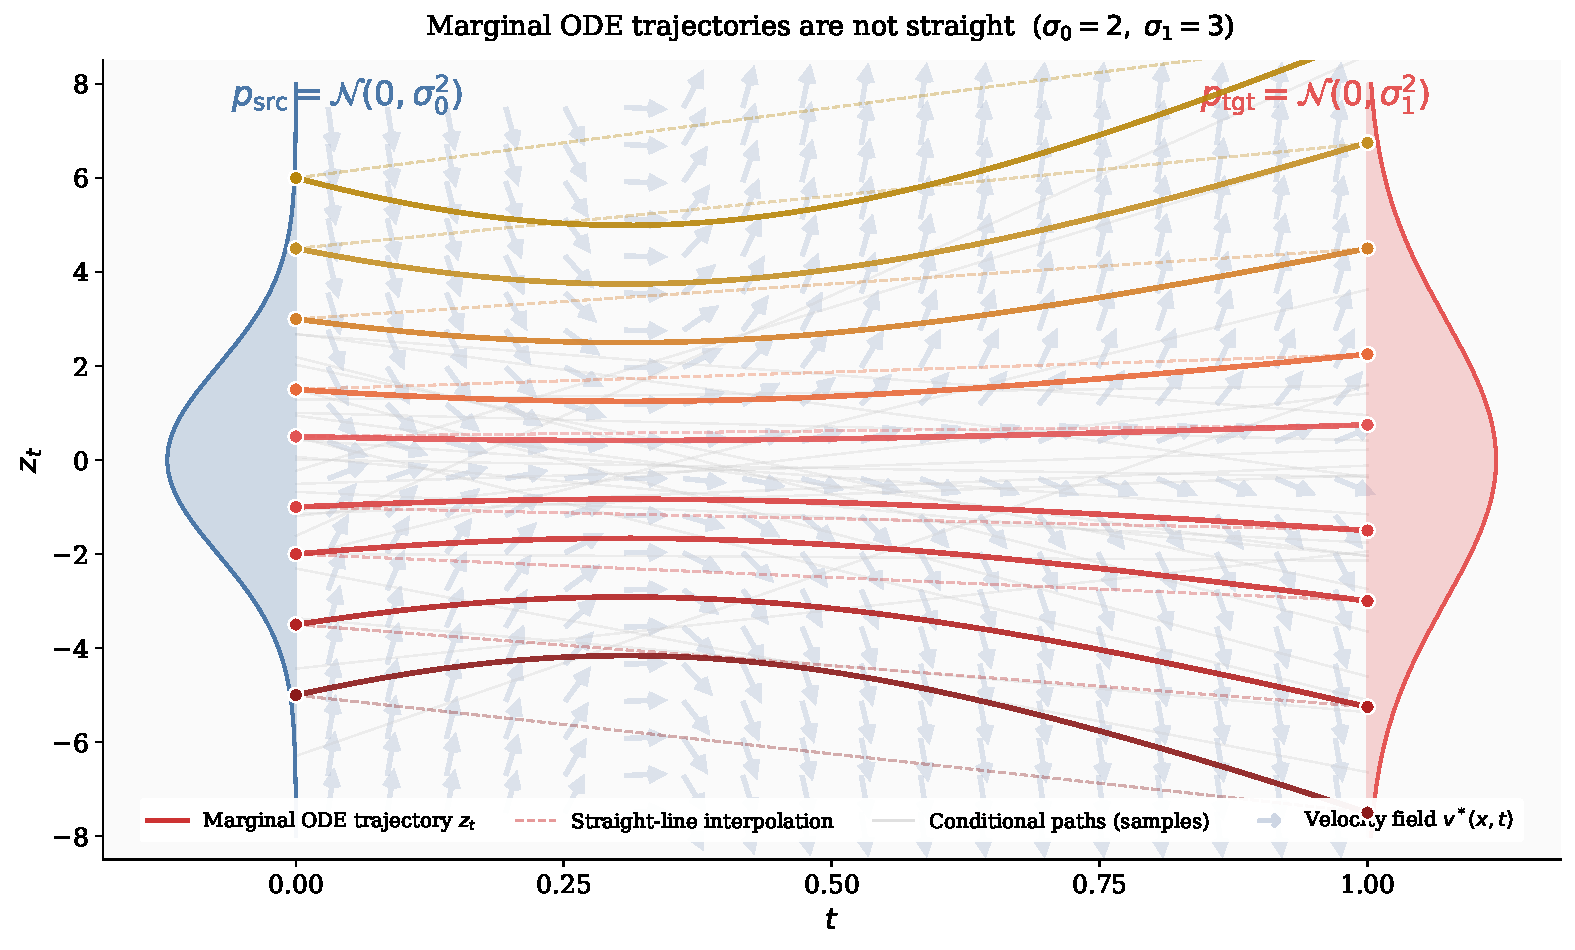
\includegraphics[width=\linewidth]{Images/PartB/straightness_counterexample.pdf}
    \caption{\textbfs{Marginal ODE trajectories are not straight under the canonical affine interpolation.}
    We take $x_0 \sim \mathcal{N}(0, \sigma_0^2)$ and $x_1 \sim \mathcal{N}(0, \sigma_1^2)$ with $\sigma_0=2$, $\sigma_1=3$, and independent coupling.
    Gray lines show sampled conditional paths $(1-t)x_0 + tx_1$, which are straight by construction.
    Solid curves show the exact marginal ODE trajectories $z_t = z_0\sqrt{(1-t)^2 + (\sigma_1/\sigma_0)^2 t^2}$, and dashed lines show the corresponding straight-line interpolations from $z_0$ to $z_1$.
    The visible gap between solid and dashed curves confirms that the marginal ODE trajectories are not affine in $t$, even though every conditional path is a straight line.
    The marginal densities $p_{\mathrm{src}}$ and $p_{\mathrm{tgt}}$ are shown on the left and right margins, respectively.
    \figcredit{Created by the authors with AI-assisted coding.}}
\end{figure}
     





%%%%%%%%%%%%%%%%%%%%%%%%%%%%%%%%%%%%%%%%%%%%%%%%%%%%%%%%%%%%%%%%%%%%%%%%
\clearpage
\newpage
%%%%%%%%%%%%%%%%%%%%%%%%%%%%%%%%%%%%%%%%%%%%%%%%%%%%%%%%%%%%%%%%%%%%%%%%

S\section{\texorpdfstring{(Optional) Properties of the Canonical Affine Flow}{(Optional) Properties of the Canonical Affine Flow}}\label{sec:optimal-canonical}

Given two endpoint distributions $p_0=p_{\mathrm{src}}$ and $p_1=p_{\mathrm{tgt}}$, 
a natural and widely used choice for defining the conditional path in flow matching (FM)~\citep{lipman2022flow} 
and rectified flow (RF)~\citep{liu2022flow} is the linear interpolation
\[
a_t = 1 - t, \qquad b_t = t,
\]
which yields the interpolant
\[
\mathbf{x}_t = (1 - t)\mathbf{x}_0 + t \mathbf{x}_1, 
\qquad \mathbf{x}_0 \sim p_{\mathrm{src}},\ \mathbf{x}_1 \sim p_{\mathrm{tgt}}.
\]
Under this choice, the training objective simplifies to
\[
\mathbb{E}_{t \sim \mathcal{U}[0,1]}   
\mathbb{E}_{\mathbf{x}_0, \mathbf{x}_1} 
\left[ \bigl\|\mathbf{v}_{\bm{\phi}}(\mathbf{x}_t, t) - (\mathbf{x}_1 - \mathbf{x}_0)\bigr\|_2^2 \right].
\]

This linear flow enjoys several appealing properties. 
In particular, it admits an iterative refinement scheme, known as \emph{\texttt{Reflow}}, 
which progressively straightens the path between distributions while preserving the marginals. 





\subsection{Rectifying Flows: From Noisy Guesses to Structured Pairings}\label{subsec:rectify}

\paragraph{From Noise to Data via Coherent Paths.}
Take the generation task where $p_{\text{src}}$ is the prior and $p_{\text{tgt}}$ is the real data. We want a continuous path that transports noise to data. A naive tactic samples $\rvz_0 \sim p_{\text{src}}$ and $\rvx_1 \sim p_{\text{tgt}}$ independently, interpolates (e.g.\ $\rvx_t=(1-t)\rvx_0+t\rvx_1$), and fits a velocity field to that line. This creates \emph{incoherent pairings}: endpoints are unrelated across iterations, so trajectories fluctuate, variance explodes, convergence slows, and sample quality suffers.

\paragraph{Why Independent Couplings Fall Short.}
Conditional flow matching with independent draws uses
\[
\pi(\rvz)=p_{\text{src}}(\rvx_0) p_{\text{tgt}}(\rvx_1),
\]
or one-sided variants. Such couplings are sampling-friendly but induce jagged, high-variance paths that a velocity field struggles to model.

\paragraph{Rectify the Flow via Dependent Coupling.}
Rather than relying on arbitrary pairings, we use a pre-trained diffusion model $\rvv_{\bphi^\times}(\cdot,t)$ as the drift in a PF-ODE to \emph{deterministically} transport each source point. Starting from $\rvz(0)=\rvz_0 \sim p_{\text{src}}$, we integrate
\[
\frac{\diff \rvz(t)}{\diff t} = \rvv_{\bphi^\times}(\rvz(t),t), \qquad t \in [0,1],
\]
to obtain $\hat\rvz_1 := \rvz(1)$ positioned near the data space learned from the pre-trained model. The resulting pair $(\rvz_0,\hat\rvz_1)$ forms a \emph{dependent coupling}: it follows a structured, model-guided path rather than an arbitrary interpolation. This idea extends naturally to affine reference paths of the form $\rvx_t = a_t \rvx_0 + b_t \rvx_1$, where $\rvx_0 \sim p_{\text{src}}$ and $\rvx_1 \sim p_{\text{tgt}}$.



\begin{algorithm}[H]
\caption{\texttt{Rectify} Operation\label{alg:Rectify}}
\begin{algorithmic}[1]
\Require Reference path $\{\rvx_t\}_{t\in[0,1]}$ (e.g.\ $\rvx_t=a_t\rvx_0+b_t\rvx_1$)
\State \textbfs{Pre-Train Diffusion.} Fit $\rvv_{\bphi^\times}$ on the chosen path by minimizing
\[
\bphi^\times \in \arg\min_{\bphi} 
\mathbb{E}_{t,\rvx_0,\rvx_1} \left[\Big\|\rvv_{\bphi}(\rvx_t,t)-\frac{\diff \rvx_t}{\diff t}\Big\|_2^2\right].
\]
\State \textbfs{Rectify.} Sample $\rvz_0 \sim p_{\text{src}}$ and integrate
\[
\frac{\diff \rvz(t)}{\diff t}=\rvv_{\bphi^\times}(\rvz(t),t),\qquad \rvz(0)=\rvz_0,\quad t\in[0,1],
\]
to obtain $\hat\rvz_1=\rvz(1)$ and the trajectory $\{\rvz(t)\}_{t\in[0,1]}$.
\Ensure Dependent (coherent) pair $(\rvz_0,\hat\rvz_1)$ or the full trajectory.
\end{algorithmic}
\end{algorithm}

\paragraph{Why It Works: Marginal-Preserving Structure.}
Let $\bPhi_{0\to t}$ denote the flow map generated by the above ODE defined by the pre-trained diffusion $\rvv_{\bphi^\times}$; then $\rvz(t)=\bPhi_{0\to t}(\rvz_0)$ and $\hat\rvz_1=\bPhi_{0\to 1}(\rvz_0)$. The \texttt{Rectify} procedure pairs each source point with its flow endpoint, giving the deterministic joint
\[
\pi_{\text{Rectify}}(\rvz_0,\rvz_1)
= p_{\text{src}}(\rvz_0) \delta \big(\rvz_1-\bPhi_{0\to 1}(\rvz_0)\big).
\]
We have two immediate consequences:
\begin{itemize}
    \item \textbfs{Source Marginal is Preserved:} 
    $\displaystyle \int \pi_{\text{Rectify}}(\rvz_0,\rvz_1) \diff \rvz_1
    = p_{\text{src}}(\rvz_0)$.
    \item \textbfs{Pushforward Along the Flow:} 
    $\displaystyle (\bPhi_{0\to t})_{\#}p_{\text{src}}=\mathrm{Law}(\rvz(t))$, i.e., the time–$t$ distribution is the pushforward of $p_{\text{src}}$ by $\bPhi_{0\to t}$.
\end{itemize}
If $\rvv_{\bphi^\times}$ matches the oracle drift of a given reference path $\rvx_t$, then all intermediate marginals coincide:
\[
\mathrm{Law}(\rvz(t))=\mathrm{Law}(\rvx_t),\quad \text{for all }t\in[0,1],
\quad\text{and}\quad
(\bPhi_{0\to 1})_{\#}p_{\mathrm{src}}=p_{\mathrm{tgt}}.
\]


\paragraph{Summary.}
Rectification replaces noisy independent pairings with smooth teacher-guided trajectories, lowering variance, easing optimization, and improving samples. The idea covers canonical linear paths $\rvx_t=(1-t)\rvx_0+t\rvx_1$ and general affine forms $\rvx_t=a_t\rvx_0+b_t\rvx_1$.

For the canonical path, repeatedly applying \texttt{Rectify} (``\emph{\texttt{Reflow}}'') further straightens trajectories without increasing transport cost, making training still easier.




\subsection{\texttt{Reflow}: Iteratively Straightening Flows}\label{subsec:reflow-def}

\paragraph{Why \texttt{Reflow}?}
Independent pairings often induce irregular and meandering ODE trajectories between $p_{\text{src}}$ and $p_{\text{tgt}}$, which increase discretization error and variance during simulation. This raises a natural question:

\begin{question}\label{ques:straight}
Can we learn couplings that induce transport paths that are closer to straight lines between the two distributions, while still preserving the correct marginals?
\end{question}

This motivates \emph{\texttt{Reflow}}: repeatedly apply \texttt{Rectify} to update the coupling so that successive flows become easier to integrate.

\paragraph{Core Idea: Recursive Straightening via \texttt{Rectify}.}
Start from the canonical interpolation on the product coupling $\pi^{(0)}:=p_{\text{src}}(\rvx_0)p_{\text{tgt}}(\rvx_1)$,
\[
\rvx_t = (1-t) \rvx_0 + t \rvx_1.
\]
Applying \texttt{Rectify} replaces the independent pairing with a dependent one $(\rvz_0,\hat\rvz_1)$, which empirically induces \emph{lower-curvature} trajectories under the learned field. Iterating this update progressively reduces path curvature (never forcing literal straight lines), improving numerical stability and alignment.

\paragraph{The \texttt{Reflow} Procedure.}
Each iteration performs two steps:
\begin{itemize} 
    \item \textbfs{Re-Fit Flow:} Train a new velocity field from samples of the current coupling: \begin{align} \bm{\phi}_{k+1} &= \arg\min_{\bm{\phi}} \mathcal{L}\left(\bm{\phi}\Big\vert \pi^{(k)}\right), \quad \text{where} \notag \\ \mathcal{L}\left(\bm{\phi}\Big\vert \pi^{(k)}\right) &:= \mathbb{E}_{t, (\rvz_0^{(k)}, \hat\rvz_1^{(k)})\sim \pi^{(k)}} \left[\left\|\rvv_{\bm{\phi}}(\rvz_t, t) - (\hat\rvz_1^{(k)} - \rvz_0^{(k)})\right\|^2\right] \label{eq:reflow-loss} \end{align} with $\rvz_t = t \rvz_0^{(k)} + (1 - t) \hat\rvz_1^{(k)}$. 
    \item \textbfs{Generate New Coupling:} Solve the learned ODE starting from new source samples $\rvz_0^{(k+1)} \sim p_{\text{src}}$: \[ \hat\rvz_1^{(k+1)} \gets \rvz_0^{(k+1)} + \int_0^1 \rvv_{\bm{\phi}_{k+1}}(\rvz(t), t) \mathrm{d}t, \] and define the updated coupling: \[ \pi^{(k+1)}(\rvz_0, \rvz_1) := p_{\text{src}}(\rvz_0) \delta\left(\rvz_1 - \hat\rvz_1^{(k+1)}\right). \] \end{itemize}
In other words, \texttt{Reflow} can be viewed as repeatedly applying the \texttt{Rectify} operator, producing a sequence of progressively refined couplings:
\begin{align}\label{eq:rectify-op}
    \pi^{(k+1)} = \texttt{Rectify} \left(\pi^{(k)}\right)
\end{align}
so that both the flow and the coupling evolve together, yielding progressively more stable transport paths.



\subsection{Properties of \texttt{Reflow}}\label{subsec:reflow-properties}

Two key theoretical properties drive the usefulness of \texttt{Reflow}: it reduces transport cost and it straightens the trajectories.

\paragraph{I. \texttt{Reflow} Never Increases Transport Cost.}
Let $c(\rvy)$ be a convex cost function (e.g., $\|\rvy\|_2^p$ with $p \geq 1$). Each \texttt{Rectify} step forms a new coupling $(\rvz_0, \hat\rvz_1)$ whose cost is no worse than the original:
\proppp{\texttt{Rectify} May Reduce Transport Costs}{rec-transport-cost}{
Assuming an ideal velocity field $\rvv^* = \rvv_{\bm{\phi}^\times}$, we have:
\[
\mathbb{E}\left[c\left(\hat\rvz_1 - \rvz_0\right)\right] \leq \mathbb{E}\left[c\left(\rvx_1 - \rvx_0\right)\right].
\]
}{Follows from Jensen's inequality. See \citet{liu2022flow} for a full derivation.}
Applying this result recursively shows that the \texttt{Reflow} process does not increase the transport cost.

\paragraph{II. \texttt{Reflow} Straightens the Path.}
The longer we iterate \texttt{Reflow}, the straighter the learned trajectories may become. To measure this, define the \emph{straightness functional} of a path $\mathbf{Y} = \{\rvy_t\}_{t\in[0,1]}$ as
\[
\mathcal{S}(\mathbf{Y}) := \int_0^1 \mathbb{E}\left[\left\|\rvy_1 - \rvy_0 - \frac{\mathrm{d}\rvy_t}{\mathrm{d}t} \right\|_2^2 \right]  \mathrm{d}t.
\]
If $\mathcal{S}(\mathbf{Y}) = 0$, then $\mathbf{Y}$ is exactly a straight line.

\proppp{\texttt{Reflow} Straightens the Stochastic Path}{reflow-straight}{
For rectified paths $\rmZ^{(k)}$, we have:
\[
\min_{k \in \{0,\dots,K\}} \mathcal{S}(\rmZ^{(k)}) \leq \frac{\mathbb{E}\left[\|\rvx_1 - \rvx_0\|^2\right]}{K}.
\]
}{See Theorem 3.7 of \citet{liu2022rectified}.}

\begin{figure}[t]
    \centering
    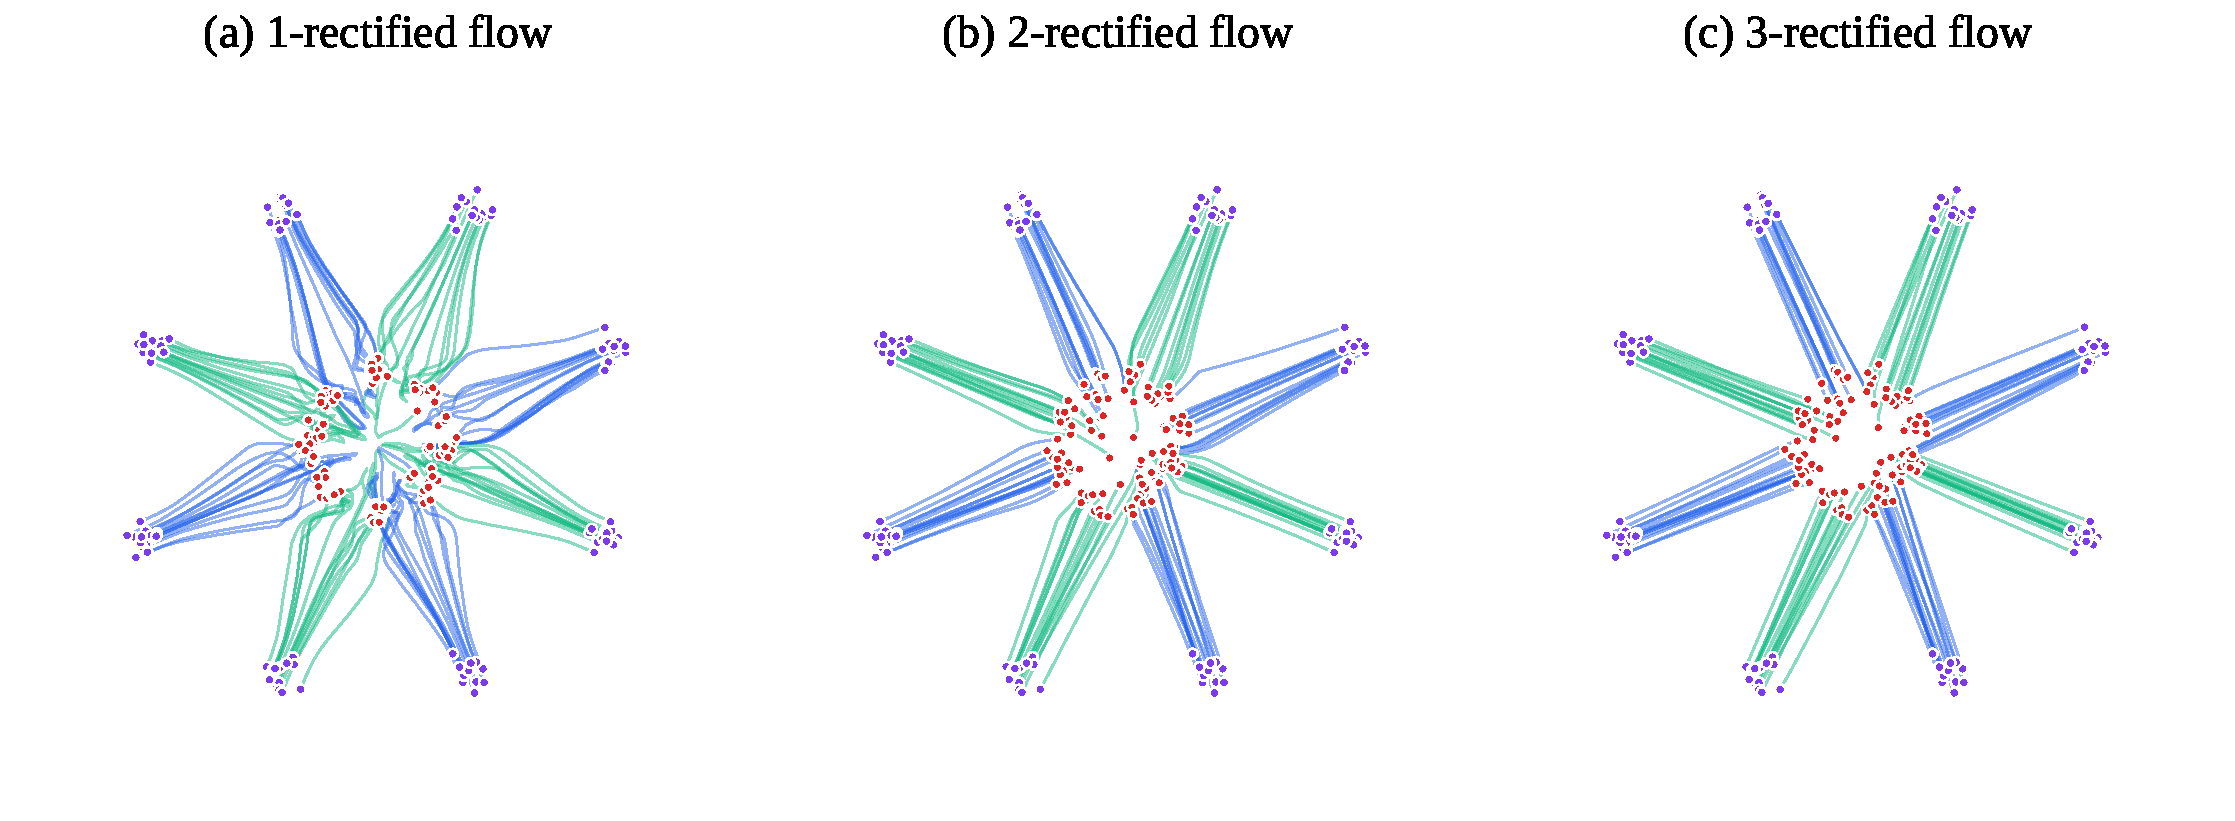
\includegraphics[width=\textwidth]{Images/PartB/rectified_flow_trained.pdf}
    \caption{\textbfs{Illustration of \texttt{Reflow}.} Paths become progressively straighter with \texttt{Rectify} procedure.  \figcredit{Adapted from \citet{liu2022flow}.}}
    \label{fig:ill_Reflow}
\end{figure}


The FM or RF formulation with linear interpolation kernels, together with the \texttt{Reflow} procedure, provides a simpler training objective and a practical method for refining stochastic couplings. For theoretical details, we refer readers to \citep{liu2022flow, liu2022rectified}.



\paragraph{III. Connection to Optimal Transport.}
Lastly, we note that straight-line couplings are not necessarily optimal in the sense of optimal transport (OT). This involves some terminology that will be introduced in \Cref{sec:ot-intro}; we therefore refer readers who are not familiar with OT to that section.

A hallmark of quadratic-cost optimal transport is that particles travel along straight lines: a particle at $\rvx_0$ moves to $\rmT(\rvx_0)$ via $\rvx_t = (1 - t)\rvx_0 + t \rmT(\rvx_0)$, where $\rmT$ is the optimal transport map. However, not every map $\rmS$ generating such straight-line paths, i.e., $\rvx_t = (1 - t)\rvx_0 + t \rmS(\rvx_0)$, is optimal. The map $\rmS$ yields the optimal flow only if it minimizes the Monge cost $\mathbb{E}[\|\rvx_0 - \rmS(\rvx_0)\|^2]$. Thus, while straight-line paths are necessary, they are not sufficient; optimality also depends on the correct endpoint map $\rmT$.

\exm{Straight Couplings Need Not Be Optimal}{
Let $p_{\text{src}} = p_{\text{tgt}} = \mathcal{N}(\bm{0}, \rmI)$. For the cost $c(\rvx, \rvy) = \|\rvx - \rvy\|^p$ with $p > 0$, the $c$-optimal coupling is the identity coupling $\pi^{*}$, where $\pi^{*}$ is the law of $(\rvx, \rvx)$ with $\rvx \sim p_{\text{src}}$.

Now consider the coupling $\pi_{\rmA}$ defined as the law of $(\rvx, \rmA \rvx)$, where $\rvx \sim p_{\text{src}}$ and $\rmA$ is a rotation matrix satisfying $\rmA^\top \rmA = \rmI$, $\det(\rmA) = 1$, $\rmA \neq \rmI$, and $-1$ is not an eigenvalue. Then $\pi_{\rmA}$ is a valid coupling of $p_{\text{src}}$ and $p_{\text{tgt}}$, and corresponds to straight-line paths between $\rvx$ and $\rmA \rvx$, but it is not $c$-optimal for any twice-differentiable strictly convex cost $c$ with invertible Hessian. The suboptimality arises from the rotational transformation. As discussed in \Cref{eq:reflow-loss-gradient}, even removing the rotation may not lead to an optimal coupling.
}

We will continue exploring the connection to OT in \Cref{subsec:ot-linear-reflow}.

\clearpage
\newpage

\newpage
\section{Closing Remarks}\label{sec:ch5_cr}
     
This chapter has illuminated the third and final foundational perspective on diffusion models, one rooted in the principles of deterministic flows. Our exploration began with Normalizing Flows (NFs), which leverage the change-of-variables formula to learn an exact, invertible mapping between a simple prior and the data distribution. We then saw this concept evolve into a continuous-time process with Neural ODEs, where a learned velocity field governs the transformation. However, this approach comes with the significant drawback of requiring costly ODE simulations within the training loop.





The modern framework of Flow Matching (FM) was presented as an elegant and efficient solution to this challenge. By pre-defining a probability path $\{p_{t}\}_t$ and a corresponding velocity field that satisfies the continuity equation, FM establishes a clear target for the ODE flow. Crucially, just as we saw in the variational and score-based views, FM employs a powerful conditioning trick. This transforms the intractable problem of matching the marginal velocity field into a simple and tractable regression against a known conditional velocity, making training entirely simulation-free. This perspective recasts diffusion models themselves as a special case of learning a deterministic flow to transport a Gaussian prior to the data distribution.




With the introduction of the flow-based view, our survey of the three conceptual pillars of diffusion modeling is now complete. Throughout this journey, a remarkable pattern has emerged: each framework, despite its unique origins in VAEs, EBMs, or NFs, has converged on a continuous-time generative process and has relied on a conditioning strategy to enable tractable learning.

In the next chapter, we will finally synthesize these parallel threads into a single, unified framework. We will:
\begin{enumerate}
    \item Formally demonstrate that the variational, score-based, and flow-based perspectives are not merely analogous but are mathematically equivalent at a fundamental level.
    \item Show how the Fokker-Planck equation serves as the universal law governing density evolution across all three views, revealing that they are simply different lenses for describing the same core generative principle.
\end{enumerate}

This unified lens will provide a complete and systematic understanding of the modern diffusion paradigm. 



